% % % % % % % % % % % % % % % % % % % % % % % % % % % % % % % % % % % % % % % % % % % %
%                                                                                     %
% Short Sectioned Assignment LaTeX Template Version 1.0 (5/5/12)                      %
% This template has been downloaded from: http://www.LaTeXTemplates.com               %
%                                                                                     %
% Original author:  Frits Wenneker (http://www.howtotex.com)                          %
%                                                                                     %
% Modified by: Fco Javier Sueza Rodríguez (fcosueza@disroot.org)                      %
%                                                                                     %
% Changes:                                                                            %
%	    - Custom Chapters, Sections and Subsections (titlesec package)                %
%           - Document type scrbook (oneside)                                         %
%           - Use babel-lang-spanish package and marvosym                             %
%           - Use hyperref, enumitem, tcolorbox and glossaries packages               %
%           - Use Time New Roman (mathptmx), Helvetic and Courier fonts               %
%                                                                                     %
% License: CC BY-NC-SA 3.0 (http://creativecommons.org/licenses/by-nc-sa/3.0/)        %
%                                                                                     %
% % % % % % % % % % % % % % % % % % % % % % % % % % % % % % % % % % % % % % % % % % % %

%-----------------------------------------------%
%	              Packages                  %
%-----------------------------------------------%

\documentclass[paper=a4, fontsize=11pt, oneside]{scrbook}

% ---- Text Input/Output ----- %

\usepackage[T1]{fontenc}
\usepackage[utf8]{inputenc}
\usepackage{mathptmx}
\usepackage[scaled=.92]{helvet}
\usepackage{courier}
\usepackage[indent=12pt]{parskip}

\usepackage{geometry}
\geometry{verbose,tmargin=3cm,bmargin=3cm,lmargin=2.6cm,rmargin=2.6cm}

% ---- Language ----- %

\usepackage[spanish]{babel}
\usepackage{marvosym}

% ---- Another packages ---- %

\usepackage{amsmath,amsfonts,amsthm}
\usepackage{graphics,graphicx}
\usepackage{titlesec}
\usepackage{fancyhdr}
\usepackage{tcolorbox}
\usepackage{hyperref}
\usepackage{enumitem}
\usepackage[automake]{glossaries}

%--------------------------------------------------------------------%
%                      Customizing Document                          %
%--------------------------------------------------------------------%


% ----------- Custom Chapters, Sections and Subsections -------------- %

\titleformat{\chapter}[display]
			{\bfseries\Huge}
			{Tema \ \thechapter} {0.5ex}
			{\vspace{1ex}\centering}

\titleformat{\section}[hang]
			{\bfseries\Large}
			{\thesection}{0.5em}{}

\titleformat{\subsection}[hang]
			{\bfseries\large}
			{\thesubsection}{0.5em}{}

\titleformat{\subsubsection}[hang]
			{\bfseries\large}
			{\thesubsubsection}{0.5em}{}

\hypersetup{
    colorlinks=true,
    linkcolor=black,
    urlcolor=magenta
}

% ------------------- Custom heaaders and footers ------------------- %

\pagestyle{fancyplain}

\fancyhead[]{}
\fancyfoot[L]{}
\fancyfoot[C]{}
\fancyfoot[R]{\thepage}

\renewcommand{\headrulewidth}{0pt} % Remove header underlines
\renewcommand{\footrulewidth}{0pt} % Remove footer underlines

\setlength{\headheight}{13.6pt} % Customize the height of the header

% --------- Numbering equations, figures and tables ----------------- %

\numberwithin{equation}{section} % Number equations within sections
\numberwithin{figure}{section} % Number figures within sections
\numberwithin{table}{section} % Number tables within sections

% ------------------------ New Commands ----------------------------- %

\newcommand{\horrule}[1]{\rule{\linewidth}{#1}} % Create horizontal rule command


%----------------------------------------------------------------------------------------
%	TÍTULO Y DATOS DEL ALUMNO
%----------------------------------------------------------------------------------------

\title{
\normalfont \normalsize
\textsc{{\bfseries Curso 2022-2023} \\ Ciclo Superior de Desarrollo de Aplicaciones Web \\ IES Aguadulce} \\ [25pt]
\horrule{0.5pt} \\[0.4cm]
\huge Lenguajes de Marcas y Sistemas de Gestión de la Información\\
\horrule{0.5pt} \\[0.4cm]
}

\author{Francisco Javier Sueza Rodríguez}
\date{\normalsize\today}

%----------------------------------------------------------------------------------------
%                                     DOCUMENTO
%----------------------------------------------------------------------------------------

\makeglossaries
\loadglsentries{glossary.tex}

\begin{document}

\maketitle

\newpage

\tableofcontents

\newpage

\listoffigures

%\listoftables

\newpage
\chapter{Lenguajes de Marcas y Sistemas de Gestión de la Información}
En esta unidad vamos a estudiar los aspectos básicos de los lenguajes de marcas y los sistemas de gestión de la información. Por un lado, veremos la evolución de los \textbf{lenguajes de marcas}, desde GML hasta HTML, así como sus elementos y atributos, haciendo especial énfasis en XML. A continuación, veremos en que consisten los \textbf{sistemas de gestión de la información}, en concreto los \textbf{ERP}, sus características, configuración básica, personalización,..etc.

\section{Definición y Clasificación de los Lenguajes de Marcas}
Los <<lenguajes de marcas>> sirven para \textbf{codificar un documentos}. Estos incorporan \textbf{etiquetas} o marcas con \textbf{información adicional} sobre como se estructura el texto o como se presenta. El lenguaje de marcas será el que defina que etiquetas se permiten, donde deben colocarse y que significado tienen.

Todo lenguaje de marcas esta definido en un documento denominado \textbf{\gls{DTD}}, donde se establecen las marcas, los elementos utilizados por dicho lenguaje y sus correspondientes etiquetas y atributos, así como su sintaxis.

Los lenguajes de marcas se pueden clasificar, principalmente, en tres grupos:

\begin{itemize}
    \item \textbf{Orientados a la presentación}: son los utilizados generalmente por los procesadores de texto y definen como debe presentarse el documento, es decir, el formato que tiene.
    \item \textbf{De procedimientos}: orientados también a la presentación, pero en este caso, dentro de un \textbf{marco procedural} que permite la definición de macros, es decir, el programa que representa el documento debe interpretar el código en el mismo orden que aparece. Algunos ejemplos son \textbf{TeX}, \textbf{LaTeX} y \textbf{Postscript}
    \item \textbf{Descriptivos o semánticos}: estos lenguajes no describen la presentación del documento, sino que \textbf{describen la información}, que es lo que se esta representando sin especificar como debe presentarse.
\end{itemize}

Algunos ejemplos de lenguajes de marcado agrupados por su ámbito de uso son los siguientes:

\begin{itemize}
    \item \textbf{Documentación Electrónica}:
    \begin{itemize}
        \item \textbf{RTF} (Rich Text Format): fue desarrollado por Microsoft en 1987 y permite el intercambio de documentos entre los diferentes procesador de texto.
        \item \textbf{TeX}: creado por \href{https://es.wikipedia.org/wiki/Donald_Knuth}{Donald Knuth}, este lenguaje esta especialmente enfocado en la creación de textos científicos. Es considerado la mejor forma de componer formulas matemáticas complejas. \cite{tex}
        \item \textbf{Wikitexto}: permite la creación de páginas wiki en servidores preparados para soportar este lenguaje.
        \item \textbf{DocBook}: permite generar documentos separando la estructura lógica del documento de su formato, permitiendo que estos documentos puedan publicarse en diferentes formatos sin tener que modificar el documento original.
    \end{itemize}
    \item \textbf{Tecnologías de Internet}:
    \begin{itemize}
        \item \textbf{HTML},\textbf{XHTML} (Hypertext Markup Language, eXtensible Hypertext Markup Language): estos lenguajes están orientados a la creación de páginas web.
        \item \textbf{RSS} (Really Simple Sindication): permite la difusión de contenido web mediante la sindicación de contenidos.
    \end{itemize}
    \item Otros lenguajes especializados:
    \begin{itemize}
        \item \textbf{MathML} (Mathematica Markup Language): especializado en expresar los formalismos matemáticos de forma que puedan ser entendidos por diferentes aplicaciones.
        \item \textbf{VoiceXML} (Voice eXtended Markup Language): permite el intercambio de información entre usuarios y una aplicación con capacidad de reconocer el habla.
        \item \textbf{MusicXML}: permite el intercambio de partituras entre diferentes editores de partituras.
    \end{itemize}
\end{itemize}

\section{Evolución de los Lenguajes de Marcas}
A finales de los \textbf{años 60} surgen unos lenguajes informáticos, diferentes de los lenguajes de programación, orientados a la gestión de la información. Con el desarrollo de los editores y procesadores de texto surgen los primeros lenguajes informáticos orientados a la descripción y estructuración de la información: \textbf{los lenguajes de marcas}. Paralelamente también surgen otros lenguajes orientados a la representación, almacenamiento y consultar de grandes cantidades de datos: lenguajes y sistemas de bases de datos.

Los lenguajes de marcas surgieron inicialmente como lenguajes formados por un conjunto de códigos que los procesadores de textos insertaban en los documentos para dirigir el proceso de presentación (impresión) mediante una impresora. Al igual que los lenguajes de programación, estos estaban \textbf{ligados} a las características de los \textbf{procesadores de texto}y las \textbf{impresoras} en los que se usaban y no permitían a los programadores abstraerse de dichas características.

Posteriormente se añadió como medio de presentación a la pantalla y se automatizó el proceso, teniendo ya solo que pulsar una combinación teclas para lograr los resultados deseados en vez de hacerlo a mano. Este marcado estaba orientado exclusivamente a la presentación de la información, aunque posteriormente se le dieron nuevos uso surgiendo con ello el \textbf{formato generalizado}.

\subsection{El origen: GML y SGML}
Uno de los problemas que ha tenido la informática ha sido la \textbf{falta de estandarización} en los formatos de información usados por los diferentes programas.

En los años 60, \textbf{IBM} encargo a \textbf{Charles F. Goldfarb} la construcción de un sistema de edición, almacenamiento y búsqueda de documentos legales. Después de analizar el funcionamiento de la empresa se llego a la conclusión de que necesitaban un formato estándar a todos los departamentos para gestionar la documentación.

Así fue como se creó \textbf{\gls{GML}}, un formato que permitía describir los documentos de tal forma que el resultado fuese independiente de la plataforma o la aplicación utilizada. Este formato evolucionó hasta que en 1986 se creó el estándar \textbf{ISO 8879} donde se especificaba el formato \textbf{\gls{SGML}}, un lenguaje muy complejo y que requería de unas herramientas de software caras, por lo que su uso quedó relegado a grandes aplicaciones industriales.


\begin{figure}[h]
    \begin{tcolorbox}[sharp corners, colback=yellow!30, colframe=white!20]
      \scriptsize
      \begin{verbatim}
<email>
    <remitente>
        <nombre>Peter</nombre>
        <apellido>Pan</apellido>
    </remitente>
    <destinatario>
        <direccion>campanilla@paisdenuncajamas.com</direccion>
    </destinatario>
    <asunto>Paseo</asunto>
    <mensaje>¿Te apetece dar una vuelta?</mensaje>
</email>
      \end{verbatim}
    \end{tcolorbox}
\caption{Documento SGML simple}
\end{figure}

\subsection{La Popularización: HTML}

En 1990, \href{https://es.wikipedia.org/wiki/Tim_Berners-Lee}{\textbf{Tim Berners-Lee}} creó el World Wide Web y conociendo SGML, se encontró con la necesidad de compatibilizar, enlazar y organizar gran cantidad de documentos procedentes de diversos sistemas. Como solución, a partir de la sintaxis de SGML, creó un lenguaje de descripción de documentos llamado \textbf{\gls{HTML}}, combinando dos estándares ya existentes:

\begin{itemize}
    \item \textbf{\gls{ASCII}}: código basado en el alfabeto latino, tal como se usa en inglés moderno \cite{ascii}. Cualquier procesador de textos simple puede reconocer y almacenar este formato, permitiendo la transferencia de datos entre dos ordenadores.
    \item \textbf{SGML}: lenguaje que permite dar estructura al texto aplicando diferentes formatos.
\end{itemize}

\textbf{HTML} es una \textbf{versión simplificada de SGML}, ya que solo utiliza las instrucciones absolutamente necesarias. Gracias a su simplicidad, tuvo un éxito rotundo en la World Wide Web, convirtiéndose rápidamente en el \textbf{estándar general} para la \textbf{creación de páginas web}. Actualmente, HTML es el tipo de documento más utilizado en el mundo.

\begin{figure}[h]
    \begin{tcolorbox}[sharp corners, colback=yellow!30, colframe=white!20]
        \scriptsize
        \begin{verbatim}
<!DOCTYPE HTML>
<html>
    <head>
        <meta charset="utf-8" />
        <title>Ejemplo1</title>
    </head>
    <body>
        <p>Párrafo de ejemplo</p>
    </body>
</html>
        \end{verbatim}
    \end{tcolorbox}
    \caption{Documento HTML simple}
\end{figure}

\subsection{La Madurez: XML}
Uno de los problemas que surgió con HTML es que la cantidad de documentos escritos en este lenguaje creció exponencialmente, muchos de los cuales no se ceñían a ningún estándar generando bastante caos. Como respuesta es ese problema, el \textbf{\gls{W3C}} estableció en 1998 el estándar internacional \textbf{\gls{XML}}, un lenguaje de marcas puramente estructural, que \textbf{no incluye información sobre el diseño}, y permite la creación de etiquetas adaptadas a las necesidades, convirtiéndose con rapidez en el estándar para intercambio de datos en la web.

\textbf{XML} es un \textbf{\gls{metalenguaje}} con las siguientes características:

\begin{itemize}
    \item Permitir definir etiquetas propias.
    \item Permitir asignar atributos a las etiquetas.
    \item Utilizar un esquema para definir de forma exacta las etiquetas y sus atributos.
    \item La estructura y el diseño son independientes.
\end{itemize}

En realizad XML es un \textbf{conjunto de estándares} relacionados entre sí y que comprende los siguientes:

\begin{itemize}
    \item \textbf{XLS} (eXtensible Style Language): permite definir hojas de estilo para XML e incluye capacidad de transformación de documentos.
    \item \textbf{XML Linking Language}: determina aspectos sobre los enlaces entre documentos XML e incluye \textbf{Xpath}, \textbf{Xlink} y \textbf{Xpointer}.
    \item \textbf{XML Namespaces}: proveen de un contexto donde se aplican las marcas del documento XML y que se diferencian de otras con el mismo nombre válidas en otros contextos.
    \item \textbf{XML Schemas}: permiten definir restricciones que se aplicarán a un documento XML. Actualmente las mas utilizadas son \textbf{DTD}.
\end{itemize}


\begin{figure}[h]
    \begin{tcolorbox}[sharp corners, colback=yellow!30, colframe=white!20]
      \scriptsize
      \begin{verbatim}
<?xml version="1.0" encoding="UTF-8xºx"?>
<!DOCTYPE biblioteca>

<biblioteca>
    <ejemplar tipo="libro" isbn="978-2-7460-4958-1" edicion="1">
        <titulo>XML practico</titulo>
        <editorial>Ediciones Eni</editorial>
        <autor>Sebastien Lecomte</autor>
        <autor>Thierry Boulanger</autor>
        <autor funcion="traductor">Ángel Belinchon Calleja</autor>
        <prestamos>
            <lector inicio="13/05/2014" devolucion="15/05/2014">Pedro López</lector>
            <lector inicio="13/07/2015" devolucion="15/07/2015">Ali Méndez</lector>
        </prestamos>
     </ejemplar>
</biblioteca>
      \end{verbatim}
    \end{tcolorbox}
    \caption{Documento XML simple}
\end{figure}

\subsection{Comparación XML y SGML}
Aunque XML esta basado en SGML, estos tienen muchas diferencias. A continuación se muestra una tabla con las principales diferencias de estos dos lenguajes de marcas.

 \begin{table}[h]
     \centering
    {\renewcommand{\arraystretch}{1.5}
        \begin{tabular}[c]{ |l|l| }
            \hline
            \multicolumn{1}{|c|}{\textbf{XML}} & \multicolumn{1}{|c|}{\textbf{SGML}} \\ \hline
            Su uso es sencillo & Su uso es my complejo \\ \hline
            Trabaja con documentos bien formados & Solo Trabaja con documentos válidos \\ \hline
            Desarrollo de aplicaciones a bajo coste & Aplicaciones para procesarlo costosas \\ \hline
            Muy utilizado en informática y otras áreas & Se utiliza en sectores muy específicos\\ \hline
            Compatibilidad e integración con HTML & No hay compatibilidad con HTML \\ \hline
            Formateo y estilos fáciles de aplicar & Formateo y estilo relativamente complejos \\ \hline
    \end{tabular}}
 \end{table}

Como vemos en esta tabla, SGML es un un lenguaje mas complejo y costoso que XML, además de imponer mas restricciones, haciéndolo un lenguaje menos flexible que XML y mas orientado a sectores concretos. Para obtener más información sobre XML, podemos consultar el \href{https://www.w3.org/TR/REC-xml/}{Estándar XML} publicado por la W3C.

\subsection{Comparación XML y HTML}
Aunque tanto XML como HTML se crearon a partir de SGML y su sintaxis es similar, son lenguajes diferentes con propósitos diferentes, como podemos ver en la siguiente tabla.

 \begin{table}[h]
    \centering
    {\renewcommand{\arraystretch}{1.5}
        \begin{tabular}[c]{ |l|l| }
            \hline
            \multicolumn{1}{|c|}{\textbf{XML}} & \multicolumn{1}{|c|}{\textbf{HTML}} \\ \hline
            Es un perfil de SGML & Es una aplicación de SGML \\ \hline
            Permite definir conjuntos de etiquetas & Aplica un conjunto limitado de etiquetas \\ \hline
            Modelo de hiperenlaces complejo & Modelo de hiperenlaces simple \\ \hline
            Navegador como plataforma de desarrollo & Navegador como visor de páginas \\ \hline
            Compatibilidad e integración con HTML & No hay compatibilidad con HTML \\ \hline
            Fin de las etiquetas propietarias & Problema de la no compatibilidad en navegadores \\ \hline
    \end{tabular}}
\end{table}

\section{Etiquetas, Elementos y Atributos}
Los lenguajes de marcas usan una serie de etiquetas intercaladas en un documento sin formato, las cuales serán posteriormente por el interprete del lenguaje.

Existen tres términos ampliamente utilizados en los lenguajes de marcas:

\begin{itemize}
    \item \textbf{Etiquetas}: una etiqueta, también llamada \textbf{tag}, es un pequeño bloque de código que se escribe encerrado entre los símbolos \textbf{menor que} (\textbf{<}) y \textbf{mayor que} (\textbf{>}). Normalmente se utilizan \textbf{dos etiquetas}, una de \textbf{inicio} y otra de \textbf{fin}, para indicar que el efecto que queríamos conseguir ha finalizado, con la única diferencia que a la etiqueta de fin se le añade el carácter \textbf{/} antes del nombre.
    \item \textbf{Elemento}: representan estructuras mediante las que se organiza el contenido del documento, o acciones que se desencadenan cuando el navegador lo interpreta. Está \textbf{compuesto} de la \textbf{etiqueta de apertura}, la \textbf{etiqueta de cierre} y el \textbf{contenido entre ambas}.
    \item \textbf{Atributo}: es un par \textbf{nombre-valor}, que se encuentra al inicio de un elemento e indican diferentes propiedades asociadas a ese elemento
\end{itemize}

\begin{figure}[h]
    \centering
    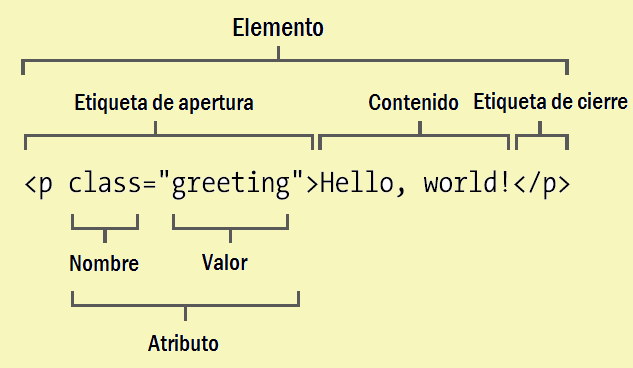
\includegraphics[scale=0.50]{elemento-HTML.png}
    \caption{Partes de un elemento HTML}
\end{figure}

\section{Herramientas de Edición}
Para trabajar con XML es necesario, por un lado, editar los documentos, y por otro procesarlos. Por ello, necesitaremos dos tipos de herramientas para trabajar con él, estas son:

\begin{itemize}
    \item \textbf{Editores XML}

    Una característica de los lenguajes de marcas es que se basan en la utilización de ficheros de \textbf{\gls{texto plano}}, por lo que basta con usar cualquier editor de texto para construir un documento XML.

    Aunque podemos usar cualquier editor, cuando elaboramos documentos XML complejos es conveniente usar
    algún software de edición XML. Estos nos ayudan a crear estructuras y etiquetas de los elementos usados en XML, resaltan las etiquetas para diferenciarlas más cómodamente y ademas incluyen ayudas para la creación de otros elementos como DTD, hojas de estilo CSS o XLS,.. El W3C ha desarrollado un editor HTML, XHTML, CSS y XML gratuito llamado Amaya, pero existen otros muchos gratuitos como: Notepad++, VSCode, Sublime Text, Netbeans,..etc

    \item \textbf{Procesadores XML}

    Para interpretar un documento XML puede usarse cualquier navegador. Los procesadores XML permiten visualizar los documentos XML y acceder a su contenido y estructura. Un \textbf{procesador} es un conjunto de módulos de software entre los que se encuentra un \textbf{parser}, que comprueba que el documento cumple las normas establecidas para que pueda abrirse. Estás normas pueden corresponderse a las necesarias para trabajar con documentos de tipo válido o solo exigir que el documento este bien formado. A los primeros se le conocen como \textbf{procesadores validadores} y a los segundos como \textbf{procesadores no validadores}.

    Para publicar documentos XML en internet se usan \textbf{procesadores XSLT}, que permiten generar archivos HTML a partir de XML.

    Puesto que XML se usa para el intercambio de archivos entre aplicaciones, hay que recurrir a motores independientes como <<XML para Java>> de IBM, JAXP de Sun, etc
\end{itemize}

\section{XML}
\textbf{XML}, que significa \textit{eXtensible Markup Language}, es un lenguaje que permite definir lenguajes de marcas desarrollado por el W3C y utilizado para almacenar datos de forma legible. Proviene del lenguaje SGML y permite definir la gramática de lenguajes específicos para estructurar documentos. \cite{xml}

Su importancia radica en que permite \textbf{compartir datos} entre diferentes equipos y aplicaciones de forma \textbf{segura}, \textbf{fiable} y \textbf{sencilla}. El hecho de que diferentes equipos y aplicaciones puedan leer y generar archivos en este formato lo convierte en una herramienta muy útil para el envío de información a través de la Web. Aunque a veces suele confundirse con HTML, podemos decir que HTML esta diseñado para mostrar datos en nuestras pantallas mientras que XML esta diseñado para almacenar y compartir esos datos.

El XML ahorra tiempos de desarrollo y proporciona ventajas, dotando a webs y aplicaciones de un método muy potente para almacenar y compartir información. Por ello, se ha convertido en un formato universal usado por todo tipo de sistemas operativos y dispositivos.

\subsection{Estructura y Sintaxis}
Un documento XML es un documento de de texto, con la \textbf{extensión .xml}, compuesto de un \textbf{conjunto de etiquetas}, \textbf{estructuradas en árbol}, que describen la organización del documento y que es interpretado por un navegador Web.

La \textbf{características básicas} de XML son las siguientes:

\begin{itemize}
    \item Es directamente \textbf{compatible} con protocolos usados en en la Web como \textbf{HTTP} y \textbf{URL}.
    \item Todo documento que verifique las reglas de XML esta \textbf{conforme con SGML}.
    \item \textbf{No se requieren conocimientos de programación} para realizar tareas sencillas en XML.
    \item Los documentos XML son\textbf{ fáciles de crear}.
    \item \textbf{La difusión} de documentos XML \textbf{está asegurada}, ya que cualquier procesador de XML puede leer documentos XML.
    \item El marcado de XML es \textbf{legible para los humanos}.
    \item El diseño de XML es \textbf{formal y conciso}.
    \item XML es \textbf{extensible}, \textbf{adaptable} y \textbf{aplicable} a una gran variedad de situaciones.
    \item XML es \textbf{orientado a objetos}
    \item Todo documento XML se \textbf{compone} de \textbf{datos de marcado} y \textbf{datos carácter} entremezclados.
\end{itemize}

El \textbf{proceso de creación} de un documento pasa por varias etapas en las que el éxito de cada una de ellas se basa en la calidad de la anterior. Estas etapas son:

\begin{enumerate}
    \item Especificación de requisitos.
    \item Diseño de etiquetas.
    \item Marcado de los documentos.
\end{enumerate}

El \textbf{marcado} son etiquetas que se añaden para estructurar los documentos y permitir a los ordenadores interpretar los textos. Los \textbf{datos carácter} son los que componen la verdad información del documento.

Los documentos XML también pueden \textbf{contener comentarios}, que son interpretados por el intérprete XML y que comienzan con la cadena \textit{<!--} y finalizan con \textit{-->}. Pueden estar en cualquier posición del documento salvo en:

\begin{itemize}
    \item El prólogo
    \item Dentro de una etiqueta
\end{itemize}

Los XML están \textbf{formados} por dos partes, \textbf{el prólogo} y \textbf{el ejemplar}, los cuales veremos a continuación.

\subsection{El Prólogo}
El prólogo es la primera parte que nos encontramos en cualquier documento XML y siempre debe preceder al ejemplar del documento. Éste se divide en dos partes, la \textbf{declaración XML} y la \textbf{declaración de la codificación} empleada, los cuales explicamos a continuación.

\begin{enumerate}
    \item\textbf{La declaración XML}: es la primera linea del documento, de no ser así, se genera un error que impide que el documento sea procesado. En caso de que sea opcional, se permite el procesamiento de documentos HTML y SGML como si fueran documentos XML, si es obligatoria, estos deberán incluir la declaración de la versión XML. Esta declaración permite indicar de forma explicita que el documento es de tipo XML.

    El prologó puede tener \textbf{tres funciones}:

    \begin{enumerate}
        \item \textbf{Declaración de la versión} utilizada de XML:
        \begin{tcolorbox}[sharp corners, colback=yellow!40, colframe=white!20]
             \begin{verbatim}               <?xml version= “1.0”?>\end{verbatim}
         \end{tcolorbox}

         \item \textbf{Declaración de la codificación empleada}:
         \begin{tcolorbox}[sharp corners, colback=yellow!40, colframe=white!20]
          \begin{verbatim}     <?xml version= “1.0” encoding=”iso-8859-1” ?>\end{verbatim}
        \end{tcolorbox}

         En este caso se usa el código código iso-8859-1 (Latin-1) que permite el uso de tildes o caracteres como la <<ñ>>. Otro de los códigos a tener en cuenta es \textbf{\gls{UTF-8}} (\textbf{\gls{unicode}}). Esta codificación soporta más caracteres que iso-8859-1 y permite que estos se visualicen correctamente en más sistemas. Es la \textbf{codificación estándar} recomendada para todos los documentos y la usaremos siempre, salvo que por algún motivo no pueda ser empleada.

         Para consultar más información sobre codificación de caracteres en sistemas informáticos y cuales son los más empleados podemos visitar  \href{https://en.wikipedia.org/wiki/Character_encoding}{página de Wikipedia} sobre codificación de caracteres.

         \item \textbf{Declaración de autonomía del documento}:

         Indica si el documento necesita de otro para su interpretación. Para declararlo, hay que definir el prólogo completo:
         \begin{tcolorbox}[sharp corners, colback=yellow!40, colframe=white!20]
             \small
             \begin{verbatim}<?xml version= “1.0” encoding=”iso-8859-1” standalone=”yes” ?>\end{verbatim}
         \end{tcolorbox}

         La opción \textit{standalone} indica al procesador XML si un documento es independiente (\textit{standalone="yes"}), o si depende de un documento externo, como declaraciones de marcas externas o una DTD externa (\textit{standalone="no"}). Por defecto el documento se considera independiente.
    \end{enumerate}

    \item \textbf{La declaración del tipo de documento}:

    Esta declaración define el tipo de documento que estamos creando para que sea procesado correctamente. Toda declaración de tipo de documento comienza con la cadena:

    \begin{tcolorbox}[sharp corners, colback=yellow!40, colframe=white!20]
        \begin{verbatim}                 <!DOCTYPE Nombre_tipo ...>\end{verbatim}
    \end{tcolorbox}
\end{enumerate}

\subsection{El Ejemplar}
Es la parte más importante de un documento XML ya que contiene los \textbf{datos reales} del documento. Es el \textbf{elemento raíz} de un documento XML y este se nombrará igual que la declaración del tipo de documento (\textit{!DOCTYPE}). Suele estar compuesto de \textbf{elementos anidados}.

En el siguiente ejemplo, el ejemplar es el elemento \textit{<libro>}, que a su vez esta compuesto de los elementos \textit{<titulo>}, \textit{<autoria>}, \textit{<editorial>}, \textit{<isbn>}, \textit{<edicion>} y \textit{<paginas>}.

\begin{figure}[h]
    \begin{tcolorbox}[sharp corners, colback=yellow!30, colframe=white!20]
        \scriptsize
        \begin{verbatim}
      <?xml version="1.0" encoding="utf-8" standalone="yes"?>
      <!DOCTYPE libro>

      <libro>
        <titulo>XML práctico</titulo>
        <autoria>
            <autor>Sebastien Lecomte</autor>
            <autor>Thierry Boulanger</autor>
        </autoria>
        <editorial>Ediciones Eni</editorial>
        <isbn>978-2-7460-4958-1</isbn>
        <edicion>1</edicion>
        <paginas>347</paginas>
      </libro>
        \end{verbatim}
    \end{tcolorbox}
    \caption{Ejemplo del \textit{ejemplar} en un documento XML}
\end{figure}

Es recomendable \textbf{establecer un criterio} y mantenerlo durante todo el documento, por ejemplo, que las etiquetas vayan escritas \textbf{siempre en minúsculas}.

Por otro lado, es conveniente anidar los elementos para una visualización óptima del documento, esto se hará \textbf{indentando} o \textbf{tabulando} el código. A continuación se muestran dos figuras, una sin indentación (errónea) y otra con indentación (correcta).

\begin{figure}[h]
    \begin{tcolorbox}[sharp corners, colback=yellow!30, colframe=white!20]
        \scriptsize
        \begin{verbatim}
        <?xml version="1.0" encoding="utf-8" standalone="yes"?>
        <!DOCTYPE libro>

        <libro>
        <titulo>XML práctico</titulo>
        <autoria>
        <autor>Sebastien Lecomte</autor>
        <autor>Thierry Boulanger</autor>
        </autoria>
        <editorial>Ediciones Eni</editorial>
        <isbn>978-2-7460-4958-1</isbn>
        </libro>
        \end{verbatim}
    \end{tcolorbox}
    \caption{Código XML sin indentación (incorrecto)}
\end{figure}

\begin{figure}[h]
    \begin{tcolorbox}[sharp corners, colback=yellow!30, colframe=white!20]
        \scriptsize
        \begin{verbatim}
        <?xml version="1.0" encoding="utf-8" standalone="yes"?>
        <!DOCTYPE libro>

        <libro>
            <titulo>XML práctico</titulo>
            <autoria>
                <autor>Sebastien Lecomte</autor>
                <autor>Thierry Boulanger</autor>
            </autoria>
            <editorial>Ediciones Eni</editorial>
            <isbn>978-2-7460-4958-1</isbn>
        </libro>
        \end{verbatim}
    \end{tcolorbox}
    \caption{Código XML con indentación (correcto)}
\end{figure}

Como podemos observar, en la segunda figura se reconoce más fácilmente la estructura del documento y se facilita la lectura de este.

Por último, es recomendable \textbf{anidar grupos de datos relacionados}, como se ha hecho en el ejemplo anterior con los elementos \textit{<autor>} dentro del elemento \textit{<autoria}, ya que el documento que \textbf{mas limpio} y \textbf{ordenado}.

\subsubsection{Elementos}
\textbf{Todos los datos} de un documento XML deben \textbf{pertenecer} a un \textbf{elemento del mismo}.

Los elementos son los diferentes \textbf{bloques de información} que permiten definir la \textbf{estructura} del documento XML. Estos está delimitados por una \textbf{etiqueta de apertura} y una \textbf{etiqueta de cierre}. Pueden estar \textbf{compuestos} por \textbf{otros elementos}.

Los \textbf{nombres} de las etiquetas deben ser \textbf{autodescriptivos}, es decir, que ilustren su contenido. Por ejemplo, si estamos con datos relativo a un libro, una etiqueta no debería ser \textit{<caracteristicas>}, ya que es demasiado ambiguo, deberíamos utilizar nombres como \textit{<titulo>}, \textit{<isbn}, etc...

La \textbf{formación de elementos} debe cumplir ciertas \textbf{normas} para que queden bien definidos y que el documento XML al que pertenecen pueda ser procesado sin generar ningún error fatal. Estas normas son las siguientes:

\begin{itemize}
    \item En todo documento XML debe existir \textbf{un documento raíz} y \textbf{solo uno}.
    \item \textbf{Todos} los elementos tienen una \textbf{etiqueta de inicio} y \textbf{otra de cierre}. En caso de que en el documento existan \textbf{elementos vacíos}, se pueden sustituir las etiquetas de apertura y cierre por una de elemento vacío. Esta se construye como una etiqueta de inicio pero añadiendo \textbf{/}, es decir, \textit{<elemento/>} en vez de \textit{<elemento>}. Esta considerada una etiqueta de apertura y cierre.
    \item Al anidar hay que tener en cuenta que \textbf{no puede cerrarse} ningún\textbf{ elemento} que \textbf{contenga otro elemento} que aún \textbf{no se haya cerrado}.
    \item Los \textbf{nombres} de las \textbf{etiquetas de apertura y cierre} deben ser \textbf{idénticos}, respetando las mayúsculas y minúsculas. Pueden ser cualquier cadena alfanumérica que no contenga espacios ni tildes, y que no comience por dos puntos (\textbf{:}), ni por la cadena \textbf{xml}.
    \item El contenido de los elementos \textbf{no puede contener} la cadena <<\textbf{\textit{]]>}}>>, por compatibilidad con SGML. Además, no se pueden utilizar los caracteres \textbf{mayor que} (\textbf{>}), \textbf{menor que} (\textbf{<}), \textbf{ampersand} (\textbf{\&}), \textbf{dobles comillas} (\textbf{"}) y \textbf{apostrofe} (\textbf{`}).

    En caso de tener que utilizar alguno de estos caracteres, se deben sustituir por las siguientes cadenas:

    \begin{table}[ht]
        \centering
        {\renewcommand{\arraystretch}{1.5}
            \begin{tabular}{ |l|l| }
                \hline
                \multicolumn{1}{|c|}{\textbf{Caracteres}} & \multicolumn{1}{|c|}{\textbf{Cadena}} \\ \hline
                \multicolumn{1}{|c|}{>} & \multicolumn{1}{|c|}{\&gt;} \\ \hline
                \multicolumn{1}{|c|}{<} & \multicolumn{1}{|c|}{<\&lt;} \\ \hline
                \multicolumn{1}{|c|}{\&} & \multicolumn{1}{|c|}{\&amp;} \\ \hline
        \end{tabular}}
         \quad
        {\renewcommand{\arraystretch}{1.5}
            \begin{tabular}{ |l|l| }
                \hline
                \multicolumn{1}{|c|}{\textbf{Caracteres}} & \multicolumn{1}{|c|}{\textbf{Cadena}} \\ \hline
                \multicolumn{1}{|c|}{"} & \multicolumn{1}{|c|}{\&quot;} \\ \hline
                \multicolumn{1}{|c|}{'} & \multicolumn{1}{|c|}{\&apos;} \\ \hline
                \multicolumn{1}{|c}{}& \\ \hline
        \end{tabular}}
     \end{table}

     \item Para \textbf{utilizar caracteres especiales}, como £, ©, ®,... hay que usar las expresiones \textit{\textbf{\&\#D;}} o \textit{\textbf{\&\#H;}}, donde D y H se corresponden con el número decimal o hexadecimal, respectivamente, correspondiente al carácter que se quiere representar en código \textbf{UNICODE}.

     En los siguientes enlaces puedes consultar tanto los códigos ASCII y su equivalente en HTML, como el código correspondiente a cada carácter en UNICODE.

     \begin{itemize}
         \item ASCII - \url{https://www.asciitable.com/}
         \item UTF-8 - \url{https://www.charset.org/utf-8}
     \end{itemize}
\end{itemize}

\subsubsection{Atributos}
Las etiquetas pueden tener \textbf{atributos}, que \textbf{permiten definir propiedades} a los elementos de un documento. Los atributos, a diferencia de los elementos, no puede organizarse en ninguna jerarquía	o estructura de árbol, no pueden contener ningún otro elemento, no pueden contener valores múltiples y no reflejan ninguna estructura lógica. En definitiva, los atributos \textbf{no se podrán extender fácilmente} en futuros cambios.

Un elemento puede tener varios atributos, pero ninguno de estos puede estar vacío, además todos los atributos dentro de un elemento \textbf{deben ser únicos}. Los atributos se codifican de la siguiente forma:

\begin{tcolorbox}[sharp corners, colback=yellow!40, colframe=white!20]
    \begin{verbatim}        <etiqueta atributo="valor_atributo"></etiqueta>\end{verbatim}
\end{tcolorbox}

No debe usarse un atributo para almacenar información susceptible de ser dividida, sino para proporcionar información adicional sobre el elemento. A continuación vamos a ver un ejemplo de la utilización de atributos en un documento XML.

\begin{figure}[h]
    \begin{tcolorbox}[sharp corners, colback=yellow!30, colframe=white!20]
        \scriptsize
        \begin{verbatim}
       <?xml version="1.0" encoding="utf-8" standalone="yes"?>
       <centro_educativo>
           <alumno sexo="Varón" fecha_nacimiento="05/06/1990">
               <nombre>Pablo</nombre>
               <apellido>Pérez</apellido>
               <telefono tipo="Móvil">666666666</telefono>
               <direccion tipo="Calle">Policar, 34</direccion>
           </alumno>
        </centro_educativo>
        \end{verbatim}
    \end{tcolorbox}
    \caption{Uso de atributos en documentos XML}
\end{figure}

Por norma general, intentaremos \textbf{evitar el uso} de atributos o procurar \textbf{no abusar de ellos}. Normalmente \textbf{los usaremos} para \textbf{metadatos} o información que no sea relevante para los datos. Se puede ver como una manera de incorporar características o propiedades a los elementos, como en el siguientes ejemplo: \textit{<perro raza=``Pastor''>Lolo</perro>}. También se suelen para especificar unidades de medida y similares: \textit{altura unidad\_altura=``cm''>178</altura>}. Hay que destacar que toda la información que se almacena en atributos se podría almacenar igualmente en elementos.

Lo que si es recomendable es que \textbf{una vez elegido un estilo}, mantenerlo dentro de todo el documento XML, teniendo en cuenta que los \textbf{nombres de los atributos} tienen que cumplir las \textbf{mismas normas} que los \textbf{elementos}, y no pueden contener el carácter menor que ``<''.

\section{Documentos XML bien formados}
Los documentos XML deben de estar \textbf{bien formados}, es decir, ser documentos \textbf{válidos}.

Los \textbf{documentos bien formados} son aquellos que cumplen las reglas sintácticas de creación de documentos XML ya mencionados en los puntos anteriores, como por ejemplo, que usan caracteres válidos para la creación de nombres de etiquetas o atributos, que las etiquetas estén cerradas correctamente, etc...

Los \textbf{documentos válidos} son aquellos que, ademas de estar bien formados, cumplen los requisitos de una definición de estructura (DTD, Schema,..), que veremos en la siguientes unidad.

Por lo tanto, para que un documento esté bien formado, debe \textbf{verificar} las \textbf{reglas sintácticas} que define la recomendación de la W3C para el \textbf{estándar XML}. Estas normas básicas se pueden resumir en las siguientes:

\begin{itemize}
    \item El documento ha de tener \textbf{definido} una \textbf{declaración XML} en el prólogo:

    \begin{tcolorbox}[sharp corners, colback=yellow!40, colframe=white!20]
        \begin{verbatim}  <?xml version="1.0" encoding="UTF-8" standalone="yes" ?>\end{verbatim}
    \end{tcolorbox}

    Hay que tener en cuenta que aunque es posible omitir el prólogo, hay navegadores que nos pueden devolver un error al procesar el documento, por lo que siempre hay que incluirlo para evitar problemas. En caso de omitirlo, los valores por defecto son los mostrados encima de este párrafo.

    \item Existe un \textbf{único elemento raíz} por cada documento: es un solo elemento en el que todos los demás contenidos y elementos se encuentran anidados.
    \item Los elementos se organizan entre sí en un \textbf{estructura jerárquica} y \textbf{no se permite} el \textbf{solapamiento} de éstos.
    \item Hay que \textbf{cumplir reglas sintácticas} a la hora de definir el nombre de elementos y atributos. Estas normas se pueden resumir en:
    \begin{itemize}
        \item El \textbf{nombre de elementos} puede contener como \textbf{primer carácter} los siguientes: \textit{[A-Z]},  \textit{[a-z]} y \textit{``\_''}. Para el resto de caracteres, ademas de estos, se pueden emplear: \textit{[0-9]}, \textit{``-''} y \textit{``.''}.
        \item Las \textbf{etiquetas de apertura y cierre} deben ser \textbf{idénticas}, teniendo en cuenta que XML es sensible a mayúsculas y minúsculas.
        \item Los \textbf{valores de los atributos} se escribirán siempre entre \textbf{comillas dobles o simples}. Si quisiéramos usar alguno de estos caracteres dentro del nombre usaríamos \&quot; (") y \&apos; ('). También hay que tener en cuenta que hay nombres reservados para el uso del lenguaje.
        \item \textbf{Los comentarios} en XML se escriben así: \textit{ <!-- Comentario -->}
    \end{itemize}
\end{itemize}

\subsection{Espacios de Nombres}
Los \textbf{espacios de nombres} permiten definir la pertenencia de los elementos y nombres a un contexto de vocabulario XML. De esta forma se resuelven las ambigüedades que se pueden producir al juntar dos documentos donde os autores han usado nombres similares para diferentes elementos.

Los espacios de nombres, también conocidos como \textbf{XML namespaces}, permiten dar nombre único a un elemento, indexándolo según un nombre de vocabulario adecuado. Además, están asociados a una \textbf{\gls{URI}}.

En el documento, las etiquetas ambiguas se sustituyen por otras con el nombre precedido de un \textbf{prefijo}, que determina el contexto al que pertenece dicho nombre:

\begin{tcolorbox}[sharp corners, colback=yellow!40, colframe=white!20]
    \begin{verbatim}       <prefijo:nombre_etiqueta></prefijo:nombre_etiqueta>\end{verbatim}
\end{tcolorbox}

Esta etiqueta de denomina \textbf{nombre cualificado}. Al definir el prefijo hay que tener en cuenta que no se pueden usar espacios ni caracteres especiales y que no puede comenzar por un dígito.

Antes de poder usar el espacio de nombres hay que declararlo, es decir, asociar un índice con la URI asignada al espacio de nombres, mediante un atributo \textbf{xmlns}. Esto se hace entre el prólogo y el ejemplar y tiene la siguientes sintaxis:

\begin{tcolorbox}[sharp corners, colback=yellow!40, colframe=white!20]
    \begin{verbatim}   <conexion>://<direccionservidor>/<apartado1>/<apartado2>/...\end{verbatim}
\end{tcolorbox}

Si queremos consultar más información acerca de los espacios de nombres, podemos consultar el estándar en la \href{https://www.w3.org/TR/REC-xml-names/}{recomendación en XML de la W3C}.

\section{Sistemas de Gestión Empresarial}
Lo primero que debemos de entender antes de meternos de lleno en los sistemas de gestión empresarial es como fluye el flujo de información en una empresa, es decir, conocer sus recursos empresariales y gestionarlos eficientemente. Estos flujos de información son los siguientes:

\begin{itemize}
    \item Entre los empleados de la empresa.
    \item Entre los empleados y la empresa.
    \item Entre la empresa con sus clientes y proveedores.
\end{itemize}

Estos \textbf{flujos de información} se puede clasificar en dos tipos:

\begin{itemize}
    \item Informales y no estructurados.
    \item Formales y estructurados, que se centran en información de procesos críticos de la empresa.
\end{itemize}

Para facilitar estos flujos de información es conveniente tener instalado un \textbf{Sistema de Información}, que facilite el conocimiento propio de la empresa para mejorar la \textbf{planificación}, la \textbf{gestión} y el \textbf{control}.

Un \textbf{Sistema de Información} se define como un conjunto organizado, de elementos relacionados, orientados  al tratamiento y administración de la información. Esta compuesto por elementos físicos, humanos y por un conjunto de normas y protocolos.

La utilización de sistema de información ofrece \textbf{ventajas competitivas} a las empresas, mejorando su eficiencia, calidad del producto o mejorando los servicios ofrecidos a los clientes. También ayudan, entre otras cosas, a la captación de clientes.

La automatización de los flujos de información cambió sustancialmente con el surgimiento de los \textbf{\gls{ERP}} y los \textbf{\gls{CRM}}, en los que se integran las diferentes aplicaciones que soportan los procesos de la empresa.

\subsection{ERP}
En una empresa, salvo que esta sea muy pequeña, es necesario usar algún sistema automatizado de gestión para controlar todos los recursos empresariales y procesos. Aquí es donde entran en juego los ERP.

Un \textbf{ERP} es un \textbf{sistema de gestión de la información} que se caracteriza por ser \textbf{una aplicación} donde hay \textbf{varias partes integradas} y se \textbf{especializa en manejar} todos los \textbf{datos relevantes} para la continuidad de la empresa. Estas partes gestionan diferentes procesos, por ejemplo producción, ventas, compras, pedidos, nóminas, etc...

Un \textbf{CRM} es un tipo de ERP que se centra en la \textbf{relación con los clientes} que tiene una empresa, es decir, información de contacto orientada a ventas.

Los \textbf{objetivos principales} de un ERP son los siguientes:

\begin{itemize}
    \item \textbf{Optimizar} los procesos empresariales.
    \item \textbf{Acceder} a la información de forma confiables y precisa.
    \item \textbf{Permitir} compartir información entre los componentes de la organización.
    \item \textbf{Eliminar} los datos y operaciones innecesarias.
\end{itemize}

Las \textbf{características} que diferencia a los ERPs de otras aplicaciones, es que deben ser \textbf{sistemas integrales}, \textbf{modulares} y \textbf{adaptables}. Sus principales características son:

\begin{itemize}
    \item Ser un programa con \textbf{acceso de una base de datos}.
    \item Sus \textbf{componentes interactúan} entre sí.
    \item Las \textbf{datos} deben ser \textbf{consistentes}, \textbf{completos}.
\end{itemize}

Suelen ser \textbf{sistemas complejos} de implantar ya que necesitan un desarrollo personalizado para las necesidades de la empresa a partir del paquete básico. Estas adaptaciones, suelen estar a cargo de \textbf{consultorías}.

Las \textbf{consultorías} en materia de \textbf{ERP} suelen ser de dos tipos:

\begin{itemize}
    \item \textbf{Consultoría de negocios}: estudia los procesos de negocio de la compañía y personaliza el ERP para ajustarlo a las necesidades de la organización.
    \item \textbf{Consultoría técnica}: estudia los recursos tecnológicos existente.
\end{itemize}

En la actualidad, la mayoría de sistemas ERP poseen \textbf{interfaz web} que mejora la accesibilidad al sistema desde prácticamente cualquier lugar y dispositivo.

\subsubsection{Características}
Las características que distinguen a un sistema de gestión empresarial son las siguientes:

\begin{itemize}
    \item \textbf{Integración}: un sistema ERP \textbf{integra todos los procesos de la empresa}, considerándolos como un serie de áreas que se relacionan entre sí para conseguir una mayor eficiencia, reduciendo tiempo y costes.
    \item \textbf{Modularidad}: \textbf{cada módulo} de un sistema ERP se corresponde con un \textbf{área funcional} de la empresa. Gracias a una \textbf{base de datos centralizada}, todos los módulos pueden compartir información entre sí, facilitando la adaptabilidad, personalización e integración. Cada módulo suele usar un software específico para su funcionalidad.
    \item \textbf{Adaptabilidad}: aunque las dos características anteriores facilitan la adaptabilidad del ERP a los requisitos de la empresa, a veces se utiliza una solución más genérica, para abaratar costes, y se modifican algunos procesos para adaptarlos al sistema ERP.
\end{itemize}

Gracias a la modularidad y la capacidad de integración de las funcionalidades, los ERPs se pueden adaptar fácilmente a las necesidades de cada empresa. Los diferentes módulos se interconectan entre sí de forma que una única herramienta ERP puede adaptarse a diferentes empresas cambiando el conjunto de módulos activos y sus relaciones.

Los \textbf{módulos principales} que forman un ERP son los siguientes:

\begin{itemize}
    \item \textbf{Ventas/Marketing}: interfaz pública que interactúa con los clientes, pedidos, estrategias de ventas, precios, promociones, publicidad, etc..
    \item \textbf{Finanzas}: es la base de cada ERP, donde se almacenan las transacciones facilitando las auditorías.
    \item \textbf{Inventario/Logística}: controla el stock y los flujos de entrada y salida.
    \item \textbf{Recursos Humanos}: gestión de personal, nómina, productividad, incentivos, etc..
    \item \textbf{Producción}: en núcleo que se encarga de los movimientos físicos del producto, planificación de materiales, etc..
\end{itemize}

Estos módulos son considerados los básicos, pero se pueden añadir muchos más como proyectos, planificación de ventas, configuración de productos a medida, etc..

No todos los \textbf{trabajadores} accederán al ERP de la misma forma, ya que cada grupo tiene su \textbf{rol}, que será supervisado por un administrador, por lo que dependiendo de este rol el trabajador tendrá unos u otros módulos habilitados.

Mención especial requieren los \textbf{CRM} (Customer Relationship Management), que surgen como consecuencia de la aplicación especifica de los ERP a las interacciones con los clientes. Están centrados en mantener, crear y potencias las relaciones con clientes sirviendo de apoyo a las políticas de marketing de la empresa.

En la actualidad los sistemas globales de CRM se pueden dividir en:

\begin{itemize}
    \item \textbf{Aplicaciones} electrónicas para los \textbf{canales de distribución} de la empresa.
    \item Centros de \textbf{atención telefónica}.
    \item \textbf{Autoservicio} para los clientes.
    \item \textbf{Gestión} electrónica de las \textbf{actividades} que afecten a los clientes.
    \item \textbf{Ventas}.
\end{itemize}

Entres sus \textbf{principales características} se encuentran la facilidad de \textbf{toma de decisiones} en \textbf{tiempo real}, \textbf{incremento de la rentabilidad} del clientes gracias a que se obtiene información muy útil a través de datos complejos, por ejemplo, identificando a los clientes que compran o que no están interesados y actuar en consecuencia.

\subsubsection{Ventajas e Inconvenientes}
Contar con un \textbf{sistema ERP personalizado}, permite a la empresa tener integradas diferentes utilidades que facilitan la gestión de la información. Aunque estos sistemas ofrecen muchas ventajas para una empresa, también tiene sus inconvenientes, como podemos ver en la siguiente lista.

\begin{itemize}
    \item \textbf{Ventajas}
    \begin{itemize}
        \item \textbf{Aumento} de la \textbf{información} que tiene la empresa sobre sus \textbf{potenciales clientes}. Los ERP que incluyen CRM aportan beneficios relacionados con la gestión de clientes de la empresa. Algunos incluyen control de calidad de los productos, permitiendo enfocar la oferta en las necesidades y deseos de los clientes, con la consecuente mejora de la satisfacción de estos.
        \item \textbf{Aumento} de las \textbf{ventas}.
        \item Permiten \textbf{resolver problemas} relacionados con el \textbf{tratamiento de la información} derivado del uso de sistemas anteriores.
        \item \textbf{Aumenta} la \textbf{eficiencia operativa}.
        \item \textbf{Facilitan} el \textbf{acceso de la información} y constituyen una mejora en las herramientas de tratamiento de la misma.
        \item \textbf{Reducción} de \textbf{costes empresariales}, especialmente los relacionados con las operaciones de las tecnologías de la información y comunicaciones.
        \item Permiten mayor \textbf{facilidad de configuración} de los sistemas de la empresa.
        \item Mejoran el \textbf{entorno de integración} de todas sus acciones.
    \end{itemize}
    \item \textbf{Inconvenientes}
    \begin{itemize}
        \item El ERP ha de ser usado y realizado por \textbf{personal capacitado}.
        \item La \textbf{instalación} del ERP es \textbf{muy costosa}.
        \item Los ERP son vistos como \textbf{sistemas muy rígidos} y difíciles de adaptar al modo de trabajo de las empresas.
        \item Son sistemas que sufren de problemas de \textbf{cuello de botella}, es decir, todos los usuarios se pueden ver afectados por la ineficiencia en uno de los departamentos.
        \item Altos \textbf{coste de modificación} de un ERP ya implantado.
    \end{itemize}
\end{itemize}

\subsubsection{ERP de Software Libre}
Dentro de los ERP de software libre encontramos una gran variedad de aplicaciones para la gestión empresarial. Entre ellas podemos destacar \textbf{Openbravo}, que es una iniciativa de origen español y \textbf{OpenERP}, actualmente conocido como \textbf{Odoo}, de origen belga y que se carateriza por tener una gran cantidad de módulos.

\textbf{Openbravo} es una aplicación de código abierto de planificación de recursos empresariales. Utiliza una arquitectura \textbf{cliente/servidor} web y esta escrita en \textbf{Java}. Se ejecuta sobre un servidor web y ofrece \textbf{soporte} para la diferentes bases de datos \textbf{Oracle} y \textbf{PostgreSQL}. Consta de dos versiones:

\begin{itemize}
    \item \textbf{Openbravo Community Edition}: versión libre y gratuita desde la que no se puede acceder a los módulos comerciales. Tiene licencia \textbf{\gls{OBPL}}.
    \item \textbf{Openbravo Network Edition}: versión bajo licencia \textbf{\gls{OBCL}} que ofrece actualizaciones de código y si ofrece acceso a los módulos comerciales.
\end{itemize}

Además de estas dos versiones, Openbravo ofrece dos soluciones diferentes:

\begin{itemize}
    \item \textbf{Suite de comercio Openbravo}: solución de comercio para minoristas.
    \item \textbf{Suite de negocio Openbravo}: solución global para empresas.
\end{itemize}

Por otro lado tenemos \textbf{Odoo} (anteriormente \textbf{OpenERP}) que resuelve problemas complejos haciendo uso de soluciones sencillas. Esta escrita en \textbf{Python} y hace uso de la base de datos \textbf{PostgreSQL}.

\textbf{OpenERP} fue creado en el año 2005 por un joven informático belga llamado \textbf{Fabien Pickaers}, causando gran sorpresa de que creara un programa de estas características y lo pusiera de forma gratuita en internet, mientras otras empresas venden sus productos a precios desorbitados. El modelo de Odoo esta basado en los servicios prestados en torno al software y tiene colaboradores alrededor de todo el mundo. En este enlace podemos ver el motivo del \href{https://openerpspain.com/}{cambio de nombre de OpenERP a Odoo}, así como la respuesta a algunas preguntas interesantes.

A continuación se muestran algunos enlaces de interese sobre estos ERPs:

\begin{itemize}
    \item \textbf{Página oficial Openbravo} - \url{www.openbravo.com/es/}
    \item \textbf{Wiki sobre OpenBravo} - \url{http://wiki.openbravo.com/wiki/Main_Page}
    \item \textbf{Página oficial de Odoo} - \url{http://www.openerp.com/es}
    \item \textbf{Doc. de usuario de Odoo} - \url{https://www.odoo.com/documentation/8.0/}
    \item \textbf{Doc. ténica de Odoo} - \url{https://www.odoo.com/documentation/user/}
\end{itemize}

\subsubsection{Instalación}
Para realizar la instalación de paquete de gestión empresarial, primero tenemos que definir \textbf{cuales} son las \textbf{necesidades que debe cubrir} el software y buscar aquel que se ajuste mejor.

En general, las \textbf{tareas} implicadas en la \textbf{instalación e implantación} de un ERP son las siguientes:

\begin{itemize}
    \item \textbf{Diseño de la instalación}: antes de iniciar la instalación deberá hacerse una análisis de cuales son las necesidades de la empresa y como las resuelve el ERP.
    \item \textbf{Instalación de equipos servidores y clientes}: será necesario revisar y actualizar el hardware de la empresa para que cumpla los requisitos el ERP.
    \item \textbf{Instalación del software}: instalación del ERP y del software que este necesite para su correcto funcionamiento.
    \item \textbf{Adaptación y migración del programa}: una vez instalado, será necesario configurarlo y adaptarlo a la empresa del cliente.
    \item \textbf{Migración de datos}: este proceso es de gran importancia ya que los datos son vitales para el correcto funcionamiento de la empresa. En ocasiones, si no hay forma de automatizar el proceso, deberá hacerse de forma manual.
    \item \textbf{Realización de pruebas}: la instalación del nuevo software puede conllevar un tiempo de transición en el que convivirá con el anterior software de gestión de la empresa. Durante este periodo de tiempo de deberán realizar pruebas para comprobar que el ERP funciona correctamente y los resultados son satisfactorios.
    \item \textbf{Documentación del sistema}: en esta fase se deben elaborar los manuales y documentos necesarios y ponerlos a disposición de la organización mediante los medios de difusión interna de los que disponga, como correo electrónico, tablón de anuncios, etc..
    \item \textbf{Formación de usuarios}: por último hay que formar a los usuarios en la utilización del ERP, empezando por los responsables de proyecto y siguiendo por los usuarios finales.
\end{itemize}

En la mayoría de los casos el sistema ERP correrán en una plataforma \textbf{cliente-servidor}, pero también pueden correr en un \textbf{servidor Web} o utilizar \textbf{tecnologías \gls{SaaS}}.

Independientemente del sistema operativo que tengamos instalado en nuestra empresa o que decidamos usar para implementar nuestro ERP, tenemos que \textbf{tener en cuenta} lo siguientes:

\begin{itemize}
    \item Tener un \textbf{servidor} donde instalaremos nuestros ERP.
    \item Instalar nuestra \textbf{base de datos} y conectarla con nuestro ERP.
    \item Instalar los \textbf{módulos necesarios ERP} que hayamos decidido adquirir.
    \item \textbf{Configurar} los diferentes \textbf{clientes} para que accedan al servidor y puedan realizar peticiones al ERP.
\end{itemize}

Hay que tener en cuenta que es \textbf{imprescindible} tener una \textbf{base de datos} instalada en nuestra empresa, ya que el sistema ERP se basa en la utilización de una base de datos para realizar los informes y las consultar. Así mismo, si decidimos incorporar el ERP a la \textbf{intranet} de la empresa será necesario disponer de un \textbf{servidor web} con soporte para el lenguaje de script en el que se haya programado la aplicación.

Los \textbf{tipos de instalación} de un sistema ERP/CRM dependerá de la plataforma con la que vayamos a trabajar con él. Los mas habituales son los siguientes:

\begin{itemize}
    \item \textbf{Instalación en máquina virtual}: la aplicaciones y programas necesarios se proporcionarán en una máquina virtual lista para su utilización. Esta opción \textbf{no es apta} para entornos de \textbf{producción}, sino que se suele usar para probar el ERP.
    \item \textbf{Instalación de paquetes en entorno gráfico}: en este caso la instalación se hace mediante el entorno gráfico del sistema operativo, usando asistentes que instalan y resuelven las dependencias de los paquetes. Aunque esta opción se puede usar en producción. los \textbf{paquetes} pueden \textbf{no estar actualizados} a la última versión.
    \item \textbf{Instalación personalizada}: si queremos instalar la versión mas reciente de la aplicación podemos descargarnos los paquetes desde la pagina web que los contenga y instalarlos de forma manual mediante comandos. Esta opción permite un mayor control sobre los paquetes que se instalan aunque también es mas compleja de llevar a cabo.
    \item \textbf{No instalar y acceder a la aplicación online}: algunos ERP nos permiten usar el software sin necesidad de instalarlo, accediendo a ir mediante internet conectándonos a un servidor que tiene todos los datos y programas de aplicación. Esta es la opción utilizada por los proveedores de ERP que ofrecen el servicio SaaS.
\end{itemize}

En \textbf{Odoo} podemos realizar diferentes tipos de instalaciones, desde paquetes, donde no tendremos que hacer prácticamente nada, hasta instalaciones paso a paso donde tendremos que instalar y configurar cada componente. Desde la \textbf{versión 8.0}, el \textbf{servicio de acceso} de \textbf{cliente de escritorio} no existe, y su acceso se \textbf{realiza} a través de un \textbf{cliente web}. Esta es la forma de acceso a la mayoría de los ERP actualmente.

\subsubsection{Personalización}
Los sistemas ERP actuales permiten la incorporación de diferentes módulos predefinidos que facilitan la personalización de la aplicación.

Un \textbf{módulo} es una aplicación que se crea para realizar una determinada función. Existen unos \textbf{módulos básicos} que se pueden cargar durante la instalación y otros que pueden instalarse posteriormente. La \textbf{integración} de estos módulos pueden realizarse durante la instalación del sistema o posteriormente durante su \textbf{ampliación}.

La integración de estos módulos se puede realizar en el momento de la instalación o posteriormente. Éstos ofrecen una una gran variedad de recursos, como creación de informes avanzados, servicios de comunicación para plataformas móviles, etc.. Hoy en día la mayoría de ERP también incluyen un modulo CRM integrado.

Para instalar los módulos hay que acceder al ERP con un usuario que tenga permisos de administrador y usar el cargador de módulos que tienen estos paquetes.

Los \textbf{principales módulos} que nos podemos encontrar en un ERP son:

\begin{itemize}
    \item \textbf{Gestión contable y financiera}: se encarga de recoger todas las operaciones contables de la compañía, centralizándolas para su consulta, publicación y control. Es módulo necesita estar integrado con un módulo de ventas para evitar duplicidades y poder acceder a los datos en tiempo real.
    \item \textbf{Compras, ventas y almacén}: el módulo de compras y ventas se encarga de registrar todas las operaciones de solicitudes de presupuestos, a proveedor, recepción de precios y creación de pedidos de compra. El módulo almacén permite gestionar las existencias de productos en almacén.
    \item \textbf{Facturación}: se encarga de generar todo tipo de información generado con la facturación de productos y servicios.
    \item \textbf{Gestión de Personal}: es módulo lleva a cabo la planificación y realización de las nominas, contratos, altas, bajas, control de horarios y datos del personal, además del sistema de pago a los empleados.
    \item \textbf{Gestión de relaciones con el cliente}: estos módulos, los \textbf{CRM}, permiten registrar todo lo relativo a la relación comercial con los clientes o posibles clientes.
\end{itemize}

En los siguientes enlaces, podemos consultar los diferentes módulos que tiene los dos ERPs que hemos tratado en esta unidad.

\begin{itemize}
    \item Módulos de Odoo - \url{https://openerpspain.com/funcionalidades-de-odoo/}
    \item Módulos de Openbravo - \url{https://www.openbravo.com/es/soluciones}
\end{itemize}

\subsubsection{Seguridad: Planificación, Usuarios y Roles}
En primer lugar, para \textbf{aumentar la seguridad} de nuestro ERP, debemos analizar los tipos de riesgos a los que está sometido. Estos se pueden clasificar en \textbf{dos tipos}:

\begin{itemize}
    \item \textbf{Riesgos Físicos}: cuando ocurre un fallo en un componente electrónico de nuestro sistema. Pueden fallar principalmente por agresiones externas, como altas temperaturas, incendios, inundaciones,etc...
    \item \textbf{Riesgos Lógicos}: sucede cuando no hay una política adecuada en los sistemas informáticos y se producen accesos no autorizados, bugs, errores en el sistema operativo o en el software, intrusiones externas, etc...
\end{itemize}

Para mitigar estos riesgos, los sistemas ERP implementan una serie de \textbf{medidas de seguridad} que se basan en los siguientes aspectos:

\begin{itemize}
    \item \textbf{Niveles de acceso configurables para los usuarios según su rol}: en función de las tareas que deba realizar un usuario, éste debe contar con una serie de políticas que le permitan acceder a los datos que necesita, quedando otros datos reservados para usuarios con un nivel de toma de decisiones mas elevado.
    \item \textbf{Auditoría de cada transacción}: se controla cada envío de datos, lo que garantiza las operaciones realizadas.
    \item \textbf{Soporte para la conexión segura con https}: para garantizar la comunicación segura entre los clientes y el servidor se usa una conexión segura. Especialmente durante el proceso de autenticación de los usuarios.
\end{itemize}

Uno de los puntos más importantes es la \textbf{buena asignación de roles}, ya que esto permite que los usuarios solo puedan acceder a los datos que necesitan dejando, restringiendo su acceso a datos más sensibles solo disponibles a usuarios con mayores privilegios. Esta asignación se realiza mediante un \textbf{usuario administrador}.

Los paquetes básicos de ERP y módulos suelen tener varios \textbf{usuarios disponibles}:

\begin{itemize}
    \item \textbf{Administrador}: es el usuario con \textbf{mayores privilegios}, tanto en el acceso a datos como en la gestión del sistema (creación de usuarios, instalación de módulos,...)
    \item \textbf{Usuario Normal}: usuario que no tiene privilegios de gestión pero si tiene acceso a \textbf{toda la información} almacenada.
    \item \textbf{Usuario Grupo}: se crean para recibir correo entrante para distribución.
    \item \textbf{Usuario de Portal}: permite a los usuarios \textbf{acceder a los portales} creados en el entorno pero \textbf{no a la aplicación}.
\end{itemize}

Hay aplicaciones en las que los usuarios no pueden borrarse directamente, sino que hay que hacerlo desde la base de datos.

Además de los diferentes usuarios, es necesario conocer las características de los \textbf{roles} que hay definidos para los usuarios de una aplicación. Estos roles definen \textbf{ciertos privilegios} a la hora de realizar \textbf{tares específicas}.

Las \textbf{características} de los \textbf{roles} son las siguientes:

\begin{itemize}
    \item Un \textbf{rol} es un \textbf{grupo particular de privilegios}.
    \item El rol solo \textbf{tiene validez} si esta \textbf{asignado a un usuario}.
    \item Un \textbf{usuario} puede tener asignados \textbf{varios roles}, en este caso prevalece el más restrictivo.
    \item Los \textbf{cambios} realizados en los roles no son \textbf{efectivos} hasta que no se \textbf{inicia sesión} de nuevo.
    \item Si un rol \textbf{niega el acceso} a un módulo, se pierde la opción de ver cualquier subpanel perteneciente a éste.
\end{itemize}


\section{Enlaces de Interés}
En esta última sección solo vamos a incluir unos enlaces para completar y aclarar algunos de los conceptos que hemos visto en esta unidad, así como para expandir un poco el contenido.

\begin{itemize}
    \item Introducción a XML - \url{https://youtu.be/bCd2xaQrTAo}
    \item Mi primer documento XML - \url{https://youtu.be/LljEw3Std1Y}
    \item Documentos XML bien formados - \url{https://youtu.be/s1RgyhO9F2I}
    \item Introducción a XML Namespaces - \url{https://youtu.be/YGFcD3-WO6c}
    \item Resumen teórico y práctico . \url{https://youtu.be/YGFcD3-WO6c}
\end{itemize}

\chapter{Definición de Esquemas y Vocabulario XML}

En este tema vamos a estudiar como establecer y definir la estructura de un documento XML. Para ello, vamos a emplear dos herramientas como son \textbf{Document Type Definition} (\textbf{DTD}) y \textbf{XML SChema Definition} (\textbf{XSD}).

Tanto DTD como XSD nos permitirán definir restricciones tanto de tipos como de estructura para un documento XML. Cada uno tiene sus ventajas he inconvenientes, las cuales estudiaremos en los siguientes puntos. También veremos algunas herramientas que nos ayudarán tanto en la creación como en la validación de documentos XML, así como de los documentos escritos en DTD o XDS.

\section{Documento XML: Estructura y Sintaxis}
Hasta ahora solo hemos trabajado con documentos XML muy básicos, los cuales podemos considera incompletos ya que solo hemos declarado que tipo de documento vamos a definir, pero no que características tiene.

Si recordamos la estructura de un documento XML que vimos en el tema anterior, este se compone de las siguientes partes:

\begin{itemize}
    \item \textbf{Prólogo}: informa al intérprete encargado de procesar el documento de todos aquellos datos que necesita para realizar su trabajo. Este consta de:
    \begin{itemize}
        \item \textbf{Definición de XML}: aquí se indica la versión de XML que se utiliza, el código de los datos a procesar y la autonomía del documento. Este ultimo dato, hasta ahora, siempre ha tenido la opción ``\textit{yes}'', ya que los documentos que hemos definido hasta ahora han sido independientes.

        \item \textbf{Declaración del tipo de documento}: hasta ahora somo hemos dicho que esta parte se compone del nombre del ejemplar precedido de la declaración ``\textit{!DOCTYPE}'' y separado de esta al menos por un espacio y seguido de  ``\textit{>}''.
    \end{itemize}

    \item \textbf{Ejemplar}: contiene los datos del documento que se quiere procesar. Es el \textbf{elemento raíz} del documento y ha de \textbf{ser único}. Esta compuesto de elementos con una estructura de árbol en la que el elemento raíz es el ejemplar y la hojas los elementos terminales, es decir, aquellos que no contienen más elementos. Los elementos, a su vez, pueden estar compuestos por atributos.
\end{itemize}

Una vez que hemos recordado la estructura básica de un documento XML, vamos a profundizar y expandir las definiciones que tenemos sobre los elementos de esta estructura y a ampliar la opciones que nos proporcionan para personalizar un documento XML.

\subsection{Declaración de Tipo de Documento}
Ya habíamos visto que esta parte nos permite establecer restricciones sobre el documento, aunque no lo habíamos profundizado en las partes que lo forman. Estas partes, se componen de los siguientes elementos:

\begin{itemize}
    \item \textbf{Declaración del tipo de documento}: comienza con el texto que indica el nombre del tipo, precedido por la cadena ``\textbf{!DOCTYPE}'' separado del nombre del tipo por al menos un espacio. El nombre del tipo debe ser idéntico al del ejemplar del documento XML en el que se ésta trabajando.

    \item \textbf{Definición del tipo de documento}: permite asociar al documento una definición de tipo \textbf{DTD}, la cual se encarga de definir las cualidades del tipo. Es decir, define los tipos de elementos, atributos y notaciones que se pueden usar en el documento, así como las restricciones del documento, valores por defecto, etc.

    Para formalizar todo esto, XML esta provisto de ciertas estructuras llamadas \textbf{declaraciones de marcado}, las cuales pueden ser internas o externas. En este último caso, deben declararse en un documento donde encontrar las declaraciones, además de indicar en la declaración de XML que el documento no es autónomo. Las diferencias entre este tipo de declaraciones de marcado dan lugar a dos subconjuntos, el \textbf{interno} y el \textbf{externo}. Durante el procesado de un documento XML, siempre se procesa primero el conjunto interno y después el externo, lo que permite sobrescribir declaraciones externas compartidas entre varios documentos y ajustar el DTD al documento específico.

    Las principales de características de los dos subconjuntos son las siguientes:

    \begin{itemize}
        \item \textbf{Subconjunto interno}: contiene las declaraciones que pertenecen a un \textbf{único documento} y no es posible compartirlas. Se localizan dentro de unos corches que siguen a la declaración del tipo de documento.

        \item \textbf{Subconjunto externo}: están localizadas en un documento con extensión \textbf{dtd} que puede situarse en el mismo directorio del documento XML. Habitualmente son declaraciones que pueden ser compartidas entre múltiples documentos XML que pertenecen al mismo tipo. En este caso, la declaración de documento autónomo ha de ser negativa, ya que es necesario el fichero con el subconjunto externo para su correcta interpretación. Esto implica que el procesado del documento se hará más lento, ya que antes de procesarlo el procesador debe obtener todas las entidades.

        Para declarar el documento externo, deberá realizarse una declaración explicita de subconjunto externo que podrá realizarse de las siguientes dos formas:

        \begin{itemize}
            \item \textbf{<!DOCTYPE nombre\_ejemplar ``URI''>}

            Se especifica una URI donde podrán localizarse las declaraciones.

            \item \textbf{<!DOCTYPE nombre\_ejemplar PUBLIC ``id\_publico'' ``URI''>}

            En este caso, también se especifica un identificador, que puede ser utilizado por el procesador para generar una URI alternativo, posiblemente basado en alguna tabla. Como se puede observar, también es necesario incluir una URI.
        \end{itemize}
    \end{itemize}
\end{itemize}

Ya que hemos visto como declarar el tipo de documento, en el siguiente punto veremos con se declara la sintaxis de un documento XML.

\subsection{Definición de Sintaxis de XML}
En los documentos de lenguajes de marcas, la distribución de los elementos esta jerarquizada según un estructura de árbol, lo que implica que es posible anidarlos pero no entrelazarlos. En este caso, el orden es significativo, pero no es así para los atributos, cuyo orden no importa, aunque si cabe recordar que no puede haber dos atributos con el mismo nombre.

Sabemos que los atributos no pueden tener nodos que dependan de ellos, por lo tanto solo pueden corresponder con las hojas de la estructura de árbol que jerarquiza los datos. Pero no solo los atributos pueden ser hojas de esta estructura, sino que los elementos pueden serlo también.

Por lo tanto, ¿que criterios podemos utilizar para decidir si un dato debe ser representado como un elemento o un atributo? Bueno, aunque no siempre se respetan, podemos tener en cuenta los siguientes criterios:

\begin{itemize}
    \item El \textbf{dato} será \textbf{un elemento} si cumple algunas de las siguientes condiciones:
    \begin{itemize}
        \item Contiene otras subestructuras.
        \item Es de tamaño considerable.
        \item Su valor cambia frecuentemente.
        \item Su valor va a ser mostrado a un usuario o aplicación.
    \end{itemize}

    \item  Un \textbf{dato} sera un \textbf{atributo}. si cumple:
    \begin{itemize}
        \item El dato es de pequeño tamaño y su valor raramente cambia, aunque hay situaciones en las que este caso se puede representar como un elemento también.
        \item El dato solo puede tener unos cuantos valores fijos.
        \item El dato guía el procesamiento de XML pero no se muestra.
    \end{itemize}
\end{itemize}

A la hora de decidir si un dato debe ser representado como atributo o elemento, por tanto, podemos comprobar si cumple unas u otras características, aunque como hemos comentado, esto no debe ser tomado como una ``guía absoluta'', ya que puede haber datos que aunque cumplan características de un atributo, pueden, o deben, ser representados como un elemento, y viceversa.

\subsubsection{XML Namespace}
Como sabemos, no puede haber atributos dentro de un mismo elemento con el mismo nombre, así como no podemos nombrar dos elementos diferentes con el mismo nombre. Para eso, XML nos proporciona los \textbf{namespaces} o \textbf{espacios de nombres}.

Un \textbf{espacio de nombre} se usan para proveer de nombres únicos a los elementos y atributos de XML, siendo su uso una recomendación de la W3C. \cite{namespace} En esencia, son una URI que referencia a una definición de vocabulario y nos permite:

\begin{itemize}
    \item Diferenciar entre los atributos y elementos de diferentes vocabularios y con diferente significado que comparten nombre.
    \item Agrupar todos los elementos y atributos de una aplicación XML para que el software pueda reconocerlos con facilidad.
\end{itemize}


Los espacios de nombres se pueden declaran usando el atributo \textbf{xmlns}, y se pueden definir de la siguiente forma.

\begin{itemize}
    \item \textbf{xmlns:``URI\_namespace''}

    \begin{figure}[h]
        \begin{tcolorbox}[sharp corners, colback=yellow!30, colframe=white!20]
            \scriptsize
            \begin{verbatim}


    <nombre xmlns="https://educacionadistancia.es/EspacioNombres">Ejemplo</nombre>
            \end{verbatim}
        \end{tcolorbox}

    \end{figure}

    \item \textbf{xmlns:prefijo=``URI\_namespace''}
    \begin{figure}[h]
        \begin{tcolorbox}[sharp corners, colback=yellow!30, colframe=white!20]
            \scriptsize
            \begin{verbatim}


<EN:nombre xmlns:EN="https://educacionadistancia.es/EspacioNombres">Ejemplo</EN:nombre>
            \end{verbatim}
        \end{tcolorbox}
    \end{figure}
\end{itemize}

En el segundo ejemplo se usa un prefijo, que nos informa de cuál es el vocabulario a la que esta asociada la definición. En ambos casos, \textbf{URI\_namespace} hace referencia al conjunto de vocabulario del espacio de nombres.

\section{Definiciones de Tipo de Documento (DTD)}
Una \textbf{definición de tipo de documento} o \textbf{DTD}, es una descripción de estructura y sintaxis de un documento XML o SGML. Su función básica es la definición de una estructura de datos, para usar un diseño común y mantener la consistencia entre los diferentes documentos que usen el mismo DTD. De esta forma, los documentos pueden ser validados, conociendo la estructura de los elementos y la descripción que trae consigo cada documento.

Así, dos o mas documentos que tengan el mismo DTD se construyen de forma similar, tienen el mismo tipo de etiquetas, en el lugar y orden que especifica el DTD.

En el tema anterior se explicó cuando un documento XML estaba bien formado o era correcto, pero un documento bien formado no es necesariamente un documento válido. Para que un documento XML sea válido tiene primero que estar bien formado, y después seguir las especificaciones dictadas por la DTD.

Las DTD \textbf{están formadas} por una \textbf{relación precisa} de \textbf{que elementos} pueden aparecer o no en el documento y \textbf{donde}, así como \textbf{el contenido} y los \textbf{atributos} de los mismos. Garantiza que los datos de un documento XML cumplen las restricciones que se le ha impuesto en el DTD, ya que éstas permiten:

\begin{itemize}
    \item \textbf{Especificar} la \textbf{estructura} del documento.
    \item Reflejar una \textbf{restricción de integridad referencial} mínima utilizando ID e IDREF.
    \item Utilizar unos pequeños mecanismos de abstracción comparables a las macro, las \textbf{entidades}.
    \item Incluir \textbf{documentos externos}.
\end{itemize}

Aunque como vemos, DTD tiene muchas ventajas, también tiene sus \textbf{inconvenientes}, siendo los principales los siguientes:

\begin{itemize}
    \item Su sintaxis \textbf{no es XML}.
    \item \textbf{No} soporta \textbf{espacio de nombres}.
    \item \textbf{No define tipos} para los datos, solo hay un tipo de elementos terminales, que son los datos textuales.
    \item\textbf{ No permite} las \textbf{secuencias no ordenadas}.
    \item \textbf{No} es posible \textbf{formar claves} a partir de \textbf{varios atributos o elementos}.
    \item Una vez que se define un DTD, \textbf{no} es posible \textbf{añadir más vocabularios}.
\end{itemize}

A continuación se muestra un ejemplo de un documento XML que queremos validar, y cual sería el resultado de aplicar un DTD que lo valide.

\begin{figure}[h]
    \begin{tcolorbox}[sharp corners, colback=yellow!30, colframe=white!20]
        \scriptsize
        \begin{verbatim}
 <?xml version="1.0"?>
 <pelicula>
 <titulo>Titanic</titulo>
 </pelicula>
        \end{verbatim}
    \end{tcolorbox}
    \caption{Documento XML que queremos validar}
\end{figure}

Con ``\textbf{!DOCTYPE pelicula /[}'' comienza la DTD y finaliza con ``\textbf{]>}''. El nombre que aparece a continuación debe ser la raíz del documento, es decir, \textbf{pelicula}, que a su vez indica que la etiqueta \textbf{titulo} esta dentro de la etiqueta \textbf{pelicula}. En la siguiente figura vemos el DTD que deberemos crear para validar este documento.

\begin{figure}[h]
    \begin{tcolorbox}[sharp corners, colback=yellow!30, colframe=white!20]
        \scriptsize
        \begin{verbatim}
<?xml version="1.0"?>
<!DOCTYPE pelicula [
<!ELEMENT pelicula (titulo)>
<!ELEMENT titulo (#PCDATA)>
]>

<pelicula>
<titulo>Titanic</titulo>
</pelicula>
        \end{verbatim}
    \end{tcolorbox}
    \caption{DTD para validar el documento}
\end{figure}

\subsection{Declaración de la DTD}
Existen dos formas de definir la DTD que describirá la estructura de un documento XML. Se puede incluir dentro del mismo documento o incluirlo en un documento externo e indicar su ubicación.

\begin{itemize}
    \item \textbf{DTD incrustada}: es posible incluir la DTD en el mismo documento, como hemos visto en el punto anterior. En la siguiente figura podemos ver un ejemplo.

    \begin{figure}[h]
        \begin{tcolorbox}[sharp corners, colback=yellow!30, colframe=white!20]
            \scriptsize
            \begin{verbatim}
<?xml version="1.0" encoding="UTF-8"?>
<!DOCTYPE pelicula [
<!ELEMENT pelicula (titulo)>
<!ELEMENT titulo (#PCDATA)>
]>
<pelicula>
<titulo>Titanic</titulo>
</pelicula>
            \end{verbatim}
        \end{tcolorbox}
        \caption{Declaración DTD incrustada}
    \end{figure}

    Cuando se declara de esta forma, se puede proporcionar una ayuda al analizador de XML, si a través de instrucciones de proceso presentes en el código, se indica que el documento es independiente y que todo lo que necesita está contenido en el mismo. Para ello, basta con añadir el atributo \textbf{standalone=``yes''}, como puede verse a continuación:

    \begin{figure}[h]
        \begin{tcolorbox}[sharp corners, colback=yellow!30, colframe=white!20]
            \scriptsize
            \begin{verbatim}


<?xml version="1.0" encoding="UTF-8" standalone="yes"?>
            \end{verbatim}
        \end{tcolorbox}
    \end{figure}

    El valor por defecto del atributo standalone es ``yes'', por lo que no sería estrictamente necesario incluirlo en este caso.

    \item \textbf{DTD externa}: otra opción es separar la declaración DTD del documento XML, realizando ésta en un documento externo e indicando donde se puede encontrar este documento. En el siguiente ejemplo, cargamos un fichero externo, \textit{cine.dtd} con la declaración DTD.

    \begin{figure}[h]
        \begin{tcolorbox}[sharp corners, colback=yellow!30, colframe=white!20]
            \scriptsize
            \begin{verbatim}
<?xml version="1.0" encoding="UTF-8" standalone="no"?> <!-- Enlace a la DTD -->
<!DOCTYPE pelicula SYSTEM "cine.dtd">
<pelicula>
<titulo>Titanic</titulo>
</pelicula>
            \end{verbatim}
        \end{tcolorbox}
        \caption{Documento SGML simple}
    \end{figure}
\end{itemize}

Aunque las dos formas de declarar un documento DTD son igual de válidas, cabe apuntar que realizar un \textbf{declaración externa} tiene ciertas \textbf{ventajas} respecto a hacerla incrustada. Algunas de estas ventajas son estas:

\begin{itemize}
    \item Si la DTD que se va a incluir es compartida por muchos documentos XML, es preferible que se encuentre en un archivo independiente, ya que si hay que hacer algún cambio en el DTD, solo tendrá que hacerse en el archivo donde este declarado, y no en cada archivo XML.

    \item La DTD puede ubicarse en un servidor web, de forma que cualquier persona con acceso a internet puede validar el documento XML que está creando, lo que garantiza que todos los documentos creados usen la última versión de la DTD. Para declarar que la DTD se encuentra en una servidor web, se puede especificar de la siguiente forma:

    \begin{figure}[H]
        \begin{tcolorbox}[sharp corners, colback=yellow!30, colframe=white!20]
            \scriptsize
            \begin{verbatim}


 <!DOCTYPE cine SYSTEM "http://cine.com/filmoteca.dtd">
            \end{verbatim}
        \end{tcolorbox}
    \end{figure}

    Aunque sería más correcto si el archivo se pusiera de forma pública. Como se muestra en el siguiente código.

    \begin{figure}[h]
        \begin{tcolorbox}[sharp corners, colback=yellow!30, colframe=white!20]
            \scriptsize
            \begin{verbatim}


<!DOCTYPE cine PUBLIC "filmoteca" "http://cine.com/filmoteca.dtd">
            \end{verbatim}
        \end{tcolorbox}
    \end{figure}

    Siendo \textbf{``filmoteca''} el nombre de la DTD.
\end{itemize}

\subsection{Declaración de Tipos de Elementos Terminales}

Los \textbf{tipos de elementos terminales} son aquellos elementos que dentro de la estructura de árbol de un documento XML serían representados por la hojas.

La declaración de tipos de elementos esta formada por la cadena ``\textbf{<!ELEMENT}'', separada por un espacio del nombre del elementos XML que se declara y seguido de la declaración de contenido de dicho elemento. En el caso de los elementos terminales, es decir, aquellos que no tienen más elementos anidados, esta declaración de contenido puede tomar los siguientes valores:

\begin{itemize}
    \item \textbf{EMPTY}: indica que el elemento no es un contenedor, es decir, que el elemento está vacío y no puede tener contenido. Para definir un elemento de este tipo se usa la siguiente definición:

        \begin{figure}[h]
        \begin{tcolorbox}[sharp corners, colback=yellow!30, colframe=white!20]
            \scriptsize
            \begin{verbatim}


      <!ELEMENT ejemplo EMPTY>
            \end{verbatim}
        \end{tcolorbox}
    \end{figure}

    \begin{itemize}
        \item XML asociado \textbf{correcto}:

     \begin{figure}[h]
        \begin{tcolorbox}[sharp corners, colback=yellow!30, colframe=white!20]
           \scriptsize
           \begin{verbatim}


       <ejemplo></ejemplo> ó <ejemplo />
           \end{verbatim}
       \end{tcolorbox}
    \end{figure}

    \item XML asociado \textbf{incorrecto}:

     \begin{figure}[h]
        \begin{tcolorbox}[sharp corners, colback=yellow!30, colframe=white!20]
            \scriptsize
            \begin{verbatim}


       <ejemplo>Esto es un ejemplo</ejemplo> ó <ejemplo><a></a></ejemplo>
            \end{verbatim}
        \end{tcolorbox}
     \end{figure}
    \end{itemize}

    \item \textbf{(\#PCDATA)}: indica que los datos son analizados en busca de etiquetas, resultando que el elemento no puede contener otros elementos, es decir, solo puede contener datos de tipo carácter, exceptuando \textbf{<}, \textbf{[}, \textbf{\&}, \textbf{]}, \textbf{>}. El elemento también podrá estar vacío. Un elemento de este tipo tendrá un definición así:

    \begin{figure}[H]
        \begin{tcolorbox}[sharp corners, colback=yellow!30, colframe=white!20]
            \scriptsize
            \begin{verbatim}


       <!ELEMENT ejemplo (#PCDATA)>
            \end{verbatim}
        \end{tcolorbox}
    \end{figure}

    \begin{itemize}
        \item XML asociado \textbf{correcto}:

        \begin{figure}[H]
            \begin{tcolorbox}[sharp corners, colback=yellow!30, colframe=white!20]
                \scriptsize
                \begin{verbatim}


       <ejemplo>Esto es un ejemplo</ejemplo> ó <ejemplo />
                \end{verbatim}
            \end{tcolorbox}
        \end{figure}

        \item XML asociado \textbf{incorrecto}:

        \begin{figure}[H]
            \begin{tcolorbox}[sharp corners, colback=yellow!30, colframe=white!20]
                \scriptsize
                \begin{verbatim}


        <ejemplo><a></a></ejemplo>
                \end{verbatim}
            \end{tcolorbox}
        \end{figure}
    \end{itemize}

    \item \textbf{ANY}: permite que el contenido de un elemento sea cualquier cosa, ya sea vacío, texto u otro elemento. \textbf{No} es \textbf{recomendable} es uso de este tipo de elemento. Para definir un elemento como ANY se usa la siguiente sentencia:

     \begin{figure}[H]
        \begin{tcolorbox}[sharp corners, colback=yellow!30, colframe=white!20]
            \scriptsize
            \begin{verbatim}


        <!ELEMENT ejemplo ANY>
            \end{verbatim}
        \end{tcolorbox}
    \end{figure}

    El problema con este tipo de dato es que no pone prácticamente restricciones al elemento, pudiendo este adoptar diferentes formas lo que hace que esta declaración de tipos sea muy poco específica. Por ejemplo, si tenemos en cuenta la siguiente declaración DTD:

    \begin{figure}[H]
        \begin{tcolorbox}[sharp corners, colback=yellow!30, colframe=white!20]
            \scriptsize
            \begin{verbatim}
       <?xml version="1.0" encoding="UTF-8"?>
       <!DOCTYPE mascota[
         <!ELEMENT mascota ANY>
         <!ELEMENT nombre (#PCDATA)>
         <!ELEMENT tipo(#PCDATA)>
          <!ELEMENT raza(#PCDATA)>
       ]>
            \end{verbatim}
        \end{tcolorbox}
    \end{figure}

    Todos los elementos que vemos a continuación, serían válidos:


        \begin{figure}[H]
        \begin{tcolorbox}[sharp corners, colback=yellow!30, colframe=white!20]
            \scriptsize
            \begin{verbatim}
        <mascota>
        <nombre>Coco</nombre> es mi mascota.
        Es una <tipo>chinchilla</tipo> <raza>blanca</raza>.
        </mascota>



        <mascota>
        Coco es mi mascota.
        Es una <tipo>chinchilla</tipo> <raza>blanca</raza>.
        </mascota>


         <mascota>
        <nombre>Coco</nombre>.
        </mascota>

        <mascota/>
            \end{verbatim}
        \end{tcolorbox}
    \end{figure}

    Por lo tanto, aunque su uso es correcto y hay determinadas situaciones en las que se debe usar, no se recomienda de forma general declarar elementos de este tipo.
\end{itemize}

\subsection{Declaración de Elementos No Terminales}
Una vez que hemos visto como declarar los elementos terminales, es decir, la hojas del árbol de la estructura, ahora vamos a ver como declarar los elementos \textbf{no terminales}, es decir, \textbf{elementos formados} por \textbf{otros elementos}, lo que serían las \textbf{ramas} del árbol de la estructura de un documento XML.

Para definir estos elementos, debemos hacer referencia a las elementos que las componen, como vemos en este ejemplo:

\begin{figure}[H]
    \begin{tcolorbox}[sharp corners, colback=yellow!30, colframe=white!20]
        \scriptsize
        \begin{verbatim}


      <!ELEMENT A(B C)>
        \end{verbatim}
    \end{tcolorbox}
\end{figure}

En este caso, se ha definido \textbf{un elemento A}, que esta \textbf{formado} por un \textbf{elemento B} seguido de un \textbf{elemento C}. Cuando un elemento aparece varias veces en un documento, también deberemos indicarlo. Para ello, se usan los siguientes operadores, que nos permiten definir la \textbf{cardinalidad} de un elemento:

\begin{itemize}
    \item \textbf{Operador opción} (\textbf{?}): este operador indica que un elemento es opcional, por lo que podrá o no aparecer en la estructura del elemento:

    \begin{figure}[H]
        \begin{tcolorbox}[sharp corners, colback=yellow!30, colframe=white!20]
            \scriptsize
            \begin{verbatim}


      <!ELEMENT telefono (trabajo? casa)>
            \end{verbatim}
        \end{tcolorbox}
    \end{figure}

    \item \textbf{Operador uno-o-más} (\textbf{+}): define un componente que aparece al menos una vez. En el siguiente ejemplo se define un elemento formado por el nombre de una provincia y otro grupo, que puede aparecer una o varias veces:

      \begin{figure}[H]
        \begin{tcolorbox}[sharp corners, colback=yellow!30, colframe=white!20]
            \scriptsize
            \begin{verbatim}


      <!ELEMENT provincia (nombre, (cp, ciudad)+ )>
            \end{verbatim}
        \end{tcolorbox}
    \end{figure}

    \item \textbf{Operador cero-o-más} (\textbf{*}): este operador permite definir un elemento que aparece cero, una o más veces. Siguiendo con el ejemplo anterior, en este caso el grupo (cp, ciudad) podría no aparecer, o hacerlo varias veces:

    \begin{figure}[H]
        \begin{tcolorbox}[sharp corners, colback=yellow!30, colframe=white!20]
            \scriptsize
            \begin{verbatim}


       <!ELEMENT provincia (nombre, (cp, ciudad)* )>
            \end{verbatim}
        \end{tcolorbox}
    \end{figure}

    \item \textbf{Operador de elección} (\textbf{|}): cuando se utiliza para sustituir las comas en la declaración de grupos indica que para formar el documento XML hay que elegir entre los elementos separados por este operador. En el siguiente ejemplo, el elemento \textit{provincia} estará formado por el elemento \textit{nombre} y el elemento \textit{cp} ó el elemento \textit{ciudad}.

    \begin{figure}[H]
        \begin{tcolorbox}[sharp corners, colback=yellow!30, colframe=white!20]
            \scriptsize
            \begin{verbatim}


      <!ELEMENT provincia (nombre, (cp | ciudad) )>
            \end{verbatim}
        \end{tcolorbox}
    \end{figure}
\end{itemize}

Ya hemos visto como se realizan las declaraciones tanto de elementos terminales como no terminales, el siguiente paso será ver como se declaran los atributos que tienen estos elementos.

\subsection{Declaración de Atributos de los Elementos}
En esta sección vamos a ver como se declaran los atributos que lleva un elemento, independientemente de si es terminal o no terminal. Para ellos, se usa la cadena \textbf{<!ATTLIST} seguida del nombre del elemento asociado al atributo que se declara, luego el nombre del atributo seguido de su tipo y modificador.

    \begin{figure}[H]
    \begin{tcolorbox}[sharp corners, colback=yellow!30, colframe=white!20]
        \scriptsize
        \begin{verbatim}


<! ATTLIST nombre_elemento nombre_atributo tipo_del_atributo "Valor_por_defecto">
        \end{verbatim}
    \end{tcolorbox}
\end{figure}

Este elemento puede usarse para declarar una lista de atributos asociados a un elemento, o repetirse el número de veces necesario para asociar a dicho elemento esa lista de atributos, pero individualmente. Si un elemento tiene más de una atributo se puede expresar de la siguiente forma:

    \begin{figure}[H]
    \begin{tcolorbox}[sharp corners, colback=yellow!30, colframe=white!20]
        \scriptsize
        \begin{verbatim}

 <! ATTLIST nombre_elemento nombre_atributo1  tipo_del_atributo1  "Valor_por_defecto"
                            nombre_atributo2  tipo_del_atributo2  "Valor_por_defecto"
                            nombre_atributo3  tipo_del_atributo3  "Valor_por_defecto"
            ........................................................................>
        \end{verbatim}
    \end{tcolorbox}
\end{figure}

Al igual que los elementos, no todos los atributos son del mismo tipo. Los tipos más destacados con los que podemos definir un atributo son los siguientes:

\begin{itemize}
    \item \textbf{Enumeración}:  con el tipo, el atributo solo podrá tomar uno de los valores especificados dentro del paréntesis, los cuales irán separados por el operador \textbf{|}. En el siguiente ejemplo, vemos que el atributo \textit{dia\_semana} solo puede tomar como valor unos de los siete días de la semana:

     \begin{figure}[H]
        \begin{tcolorbox}[sharp corners, colback=yellow!30, colframe=white!20]
            \scriptsize
            \begin{verbatim}


<!ATTLIST fecha dia_semana (lunes|martes|miércoles|jueves|viernes|sábado|domingo)>
            \end{verbatim}
        \end{tcolorbox}
    \end{figure}

    \item \textbf{CDATA}: este tipo se usa para especificar que un atributo es una cadena de texto. En el siguiente ejemplo se define el atributo \textit{color} del elemento ejemplo como CDATA:

     \begin{figure}[H]
        \begin{tcolorbox}[sharp corners, colback=yellow!30, colframe=white!20]
            \scriptsize
            \begin{verbatim}
<!ATTLIST ejemplo color CDATA #REQUIRED>

<ejemplo color="verde" />
            \end{verbatim}
        \end{tcolorbox}
    \end{figure}


    \item \textbf{ID}: permite declarar que el valor del atributo debe ser único y no se puede repetir en otros elementos ni atributos. Hay que tener en cuenta que los números no son nombres válidos en XML, por tanto no son un identificado legal.  Para resolverlo, suele incluirse un prefijo en los valores y separarlo con un guión o letra, como en el siguiente ejemplo:

    \begin{figure}[H]
        \begin{tcolorbox}[sharp corners, colback=yellow!30, colframe=white!20]
            \scriptsize
            \begin{verbatim}
<!ATTLIST libro codigo ID #REQUIRED>

<libro codigo="Q1">El Quijote</libro>
            \end{verbatim}
        \end{tcolorbox}
    \end{figure}

    \item \textbf{IDREF}: permite hacer referencia a un identificador. En esta caso, el valor del atributo ha de corresponder con el identificador de algún elemento del documento XML.

    \item \textbf{NMTOKEN}: permite definir que el valor de un atributo ha de ser solo una palabra compuesta por los caracteres permitidos en XML, es decir, letras, números y los caracteres: ``\textbf{:}'', ``\textbf{\_}'', ``\textbf{-}'' y ``\textbf{.}''.
\end{itemize}

Además de estos tipos, debemos declarar si el valor de un \textbf{atributo} es \textbf{obligatorio} o no. También podemos indicar cual será el valor por defecto de un atributo. Para todo ésto, se pueden emplear las siguiente cadenas:

\begin{itemize}
    \item \textbf{\#IMPLIED}: indica que el atributo sobre el que se aplica es opcional.

    \begin{figure}[H]
        \begin{tcolorbox}[sharp corners, colback=yellow!30, colframe=white!20]
            \scriptsize
            \begin{verbatim}
 <!ATTLIST ejemplo color CDATA #IMPLIED>

 <ejemplo color="verde" /> ó <ejemplo color="" />
            \end{verbatim}
        \end{tcolorbox}
    \end{figure}

    \item \textbf{\#REQUIRED}: indica que el atributo sobre el que se aplica es obligatorio.

      \begin{figure}[H]
        \begin{tcolorbox}[sharp corners, colback=yellow!30, colframe=white!20]
            \scriptsize
            \begin{verbatim}


 <!ATTLIST ejemplo color CDATA #REQUIRED>
            \end{verbatim}
        \end{tcolorbox}
    \end{figure}

    \begin{itemize}
        \item XML no válido:

        \begin{figure}[H]
            \begin{tcolorbox}[sharp corners, colback=yellow!30, colframe=white!20]
                \scriptsize
                \begin{verbatim}


         <ejemplo color="" />
                \end{verbatim}
            \end{tcolorbox}
        \end{figure}

        \item XML válido:

                \begin{figure}[H]
            \begin{tcolorbox}[sharp corners, colback=yellow!30, colframe=white!20]
                \scriptsize
                \begin{verbatim}


         <ejemplo color="verde" />
                \end{verbatim}
            \end{tcolorbox}
        \end{figure}
    \end{itemize}

    \item \textbf{\#FIXED}: permite definir un valor fijo para un atributo independientemente de que ese atributo se defina explícitamente en una instancia del elemento del documento XML.

          \begin{figure}[H]
        \begin{tcolorbox}[sharp corners, colback=yellow!30, colframe=white!20]
            \scriptsize
            \begin{verbatim}


  <!ATTLIST ejemplo color CDATA #FIXED "verde">
            \end{verbatim}
        \end{tcolorbox}
    \end{figure}

    \begin{itemize}
        \item XML no válido:

        \begin{figure}[H]
            \begin{tcolorbox}[sharp corners, colback=yellow!30, colframe=white!20]
                \scriptsize
                \begin{verbatim}


            <ejemplo color="rojo" />
                \end{verbatim}
            \end{tcolorbox}
        \end{figure}

        \item XML válido:

        \begin{figure}[H]
            \begin{tcolorbox}[sharp corners, colback=yellow!30, colframe=white!20]
                \scriptsize
                \begin{verbatim}


           <ejemplo color="verde" />
                \end{verbatim}
            \end{tcolorbox}
        \end{figure}
    \end{itemize}

    \item \textbf{Literal}: asigna por defecto a un atributo el valor indicado entre comillas, aunque este atributo también podrá tomar otros valores.

    \begin{figure}[H]
        \begin{tcolorbox}[sharp corners, colback=yellow!30, colframe=white!20]
            \scriptsize
            \begin{verbatim}
 <!ATTLIST ejemplo color CDATA (rojo|verde|amarillo) "verde">

 <ejemplo color="verde" />
            \end{verbatim}
        \end{tcolorbox}
    \end{figure}
\end{itemize}

Ya conocemos como se declaran los elementos y atributos en un DTD. En la siguiente sección veremos que también podemos declarar entidades, que nos ayudarán a la hora de crear este tipo de documentos.

\subsection{Declaración de Entidades}
Las entidades nos permite \textbf{declarar valores constantes} dentro de un documento XML. Cuando se emplean dentro de un documento XML se limitan por ``\textbf{`\&}'' y ``\textbf{;}''. Por ejemplo: \textbf{\&entidad}. El intérprete, al procesar el documento XML, sustituirá todas las apariciones de la entidad por el valor que se le haya asignado en el DTD. La entidades \textbf{no admiten recursividad}, es decir, una entidad no puede hacer referencia a sí misma.

Las entidades puede ser de dos tipos, \textbf{generales} y de \textbf{parámetro}.

\begin{itemize}
    \item \textbf{Entidades Generales}: dentro de la entidades generales podemos encontrar las \textbf{internas} y las \textbf{externas}:
    \begin{itemize}
        \item \textbf{Internas}: son las que se declaran  en el DTD y existen algunas predefinidas que podemos ver en la siguiente tabla.

            \begin{figure}[ht]

            \vspace{3ex}
            \centering

            \setlength{\tabcolsep}{10pt}
            \renewcommand{\arraystretch}{1.4}

            \begin{tabular}{| c | c |}
                \hline
                \textbf{Entidad}  & \textbf{Carácter} \\ \hline
                \textbf{\&lt;} &  < \\ \hline
                \textbf{\&gt;} &  > \\ \hline
                \textbf{\&guot;} &  " \\ \hline
                \textbf{\&apos;} &  ' \\ \hline
                \textbf{\&amp;} &  \& \\
                \hline
            \end{tabular}
            \caption{Entidades predefinidas en XML}
        \end{figure}

        Además de las entidades predefinidas, podemos definir las nuestras propias. Para ello emplearemos  la estructura ``\textbf{<!ENTITY nombre\_entidad ``valor entidad''>}, donde:
        \begin{itemize}
            \item \textbf{nombre\_entidad} es el nombre que recibe la entidad.
            \item \textbf{``valor\_entidad''} es el valor que toma dicha entidad.
        \end{itemize}

        Para hacer referencias a las entidades creadas usaremos \textbf{\&nombre\_entidad}.

        En la siguiente figura se puede ver un ejemplo de la definición de entidades internas propias. En este caso se declaran las entidades \textbf{autor} y \textbf{editorial}, que posteriormente se usan en el texto dentro de los elementos del documento.

        En la figura 2.2.7 podemos ver el resultado, y como el intérprete a sustituido cada ocurrencia de las entidades por sus valores en el momento de generar el documento.

       \begin{figure}[H]
           \begin{tcolorbox}[sharp corners, colback=yellow!30, colframe=white!20]
               \scriptsize
               \begin{verbatim}
<?xml version="1.0" encoding="UTF-8"?>
<!DOCTYPE libros [
<!ELEMENT libros (libro)+>
<!ELEMENT libro (#PCDATA)>

<!ENTITY autor "Miguel de Cervantes">
<!ENTITY editorial "Alfaguara">
]>


<libros>
<libro>Don Quijote de la Mancha fue escrito por &autor;</libro>
<libro>SIDI fue escrito por Arturo Pérez-Reverte y publicado por &editorial;</libro>
<libro>Tiempos recios fue escrito por Mario Vargas y publicado por &editorial;</libro>
</libros>
               \end{verbatim}
           \end{tcolorbox}
           \caption{Declaración de entidades internas en DTD}
       \end{figure}

            \begin{figure}[ht]
            \centering
            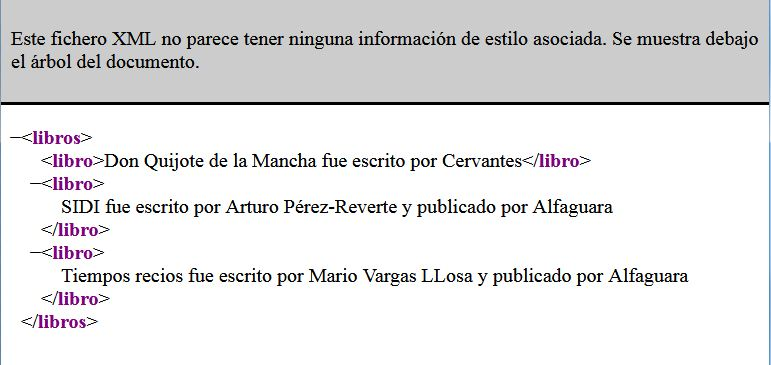
\includegraphics[scale=0.65]{dtd_entidades_internas.jpg}
            \caption{Documento generado con entidades internas sustituidas}
        \end{figure}

     \item \textbf{Externas}: permiten establece una relación entre el documento XML y otro documento a través de la URL de este último.

     \begin{figure}[h]
         \begin{tcolorbox}[sharp corners, colback=yellow!30, colframe=white!20]
             \scriptsize
             \begin{verbatim}


 <!ENTITY nombre_entidad SYSTEM "http://localhost/docsxml/fichero_entidad.xml">
             \end{verbatim}
         \end{tcolorbox}
     \end{figure}

     En este caso el contenido de los ficheros es analizado por lo que deben seguir la sintaxis XML. Cuando es necesario incluir ficheros binarios, se utiliza la palabra reservada \textbf{NDATA} en la definición de la entidad, para que el fichero no sea analizado, y habrá que asociar a dicha entidad una declaración de notación , tal y como veremos en la siguiente sección.

     En el caso de que la entidad externa vaya a ser utilizada por varias aplicaciones, deberemos declararla de la siguiente forma:

         \begin{figure}[h]
         \begin{tcolorbox}[sharp corners, colback=yellow!30, colframe=white!20]
             \scriptsize
             \begin{verbatim}


<!ENTITY nombre_entidad PUBLIC "identificador público formal" "camino hasta la DTD (uri)">
             \end{verbatim}
         \end{tcolorbox}
     \end{figure}
     \end{itemize}

    \item \textbf{Entidades de Parámetro}: al igual que la generales, éstas pueden ser \textbf{internas} y \textbf{externas}.

    \begin{itemize}
        \item \textbf{Internas}: permiten dar nombre a partes de un DTD y hacer referencias a ellas a lo largo del mismo. Son especialmente útiles cuando varios elementos del DTD comparte listas de atributos o especificaciones de contenido. Se denotan por \textbf{\%entidad}. Aquí mostramos un ejemplo de su uso.

        \begin{figure}[h]
            \begin{tcolorbox}[sharp corners, colback=yellow!30, colframe=white!20]
                \scriptsize
                \begin{verbatim}
<!ENTITY % direccion "calle, numero?, ciudad, cp">

<!ELEMENT almacen (%direccion;, web)>
<!ELEMENT oficina (%direccion;, movil)>
<!ELEMENT central (%direccion;, telefono)>
<!ELEMENT tienda (%direccion;, fax)>
                \end{verbatim}
            \end{tcolorbox}
        \end{figure}

    \item \textbf{Externas}: permite incluir en un DTD elementos externos, lo que se aplica al dividir la definición DTD en varios documentos.

            \begin{figure}[h]
        \begin{tcolorbox}[sharp corners, colback=yellow!30, colframe=white!20]
            \scriptsize
            \begin{verbatim}


 <!ENTITY %persona SYSTEM "persona.dtd">
            \end{verbatim}
        \end{tcolorbox}
    \end{figure}
    \end{itemize}
\end{itemize}

Como vemos, las entidades son bastante útiles a la hora de crear documentos DTD, y nos ayudan a establecer valores fijos para ciertos parámetro ó incluso a no tener que repetir código.

\subsection{Declaración de Notación}
En esta sección vamos a ver un tipo de declaración muy concreto que se aplica cuando queremos incluir un \textbf{fichero binario}. En este caso, deberemos indicar al intérprete que aplicación es la que se tiene que hacer cargo de procesar dicho fichero.

Para especificar la aplicación que deberá hacerse caso de ese fichero, usamos la siguiente \textbf{notación}:

\begin{figure}[h]
    \begin{tcolorbox}[sharp corners, colback=yellow!30, colframe=white!20]
        \scriptsize
        \begin{verbatim}


 <!NOTATION nombre SYSTEM aplicacion>
        \end{verbatim}
    \end{tcolorbox}
\end{figure}

Por ejemplo, en el caso de que quisiéramos incluir un archivo de tipo \textbf{gif}, donde indicáramos un editor que se encargar de visualizar este tipo de imagen, lo haríamos de la siguiente forma:

\begin{figure}[H]
    \begin{tcolorbox}[sharp corners, colback=yellow!30, colframe=white!20]
        \scriptsize
        \begin{verbatim}


 <!NOTATION gif SYSTEM "gifEditor.exe">
        \end{verbatim}
    \end{tcolorbox}
\end{figure}

En el caso de que quisiéramos asociar una entidad externa no analiza, bastaría con declarar dicha asociación de la siguiente manera:

\begin{figure}[H]
    \begin{tcolorbox}[sharp corners, colback=yellow!30, colframe=white!20]
        \scriptsize
        \begin{verbatim}


 <!ENTITY dibujo SYSTEM "imagen.gif" NDATA gif>
        \end{verbatim}
    \end{tcolorbox}
\end{figure}

Ya hemos visto todo lo relacionado con las declaraciones en DTD, por último, en el siguiente tema veremos las secciones condicionales y habremos concluido la parte dedicada a DTD.

\subsection{Secciones Condicionales}
Las \textbf{secciones condicionales} nos permiten incluir o ignorar partes de la declaración de un DTD. Para ellos se usan los dos siguientes tokens:

\begin{itemize}
    \item \textbf{INCLUDE}: permite que esta parte de la declaración sea visible. Su sintaxis es:

    \begin{figure}[H]
        \begin{tcolorbox}[sharp corners, colback=yellow!30, colframe=white!20]
            \scriptsize
            \begin{verbatim}


  <![INCLUDE [Declaraciones visibles] ] >
            \end{verbatim}
        \end{tcolorbox}
    \end{figure}

    \item \textbf{IGNORE}: permite ocultar esa sección de declaraciones dentro de DTD. Su sintaxis es:

    \begin{figure}[H]
        \begin{tcolorbox}[sharp corners, colback=yellow!30, colframe=white!20]
            \scriptsize
            \begin{verbatim}


  <![IGNORE [Declaraciones visibles] ] >
            \end{verbatim}
        \end{tcolorbox}
    \end{figure}
\end{itemize}

El uso de la secciones condicionales suele \textbf{estar ligado} al uso de \textbf{entidades paramétricas}.

\section{XML Schema}




% Glossary

\glsaddall
\printglossaries

% Bibliography

\newpage
\addcontentsline{toc}{chapter}{Bibliografía}
\bibliography{citas}
\bibliographystyle{unsrt}

\end{document}